 
%\part{Análisis de la Varianza.}
%\frame{\partpage}
%\begin{document}

\chapter{Análisis de la Varianza.}
\section{Introducción}

\begin{frame}
\frametitle{Introducción.}

\begin{itemize}
\item<2-> El análisis de la varianza (ANOVA) es una técnica para comparar medias de más de dos poblaciones. 
\item<3-> En este capítulo introduciremos aspectos elementales del diseño experimental. El diseño experimental en estadística abarca los métodos para recoger y analizar datos, cuyos objetivos son aumentar al máximo la cantidad y mejorar la exactitud de la información proporcionada por un determinado experimento. 
\item<4-> La técnica ANOVA consiste básicamente en dividir la variación total del experimento en cuestión en componentes, algunas de las cuales son debidas a la diferencia entre los distintos grupos que componen las poblaciones y las demás a variaciones aleatorias.
\end{itemize}
\end{frame}

\begin{frame}
\frametitle{Introducción}

\begin{itemize}
\item<2-> Tenemos $k$ poblaciones con una característica común que será la variable de estudio. Queremos ver si la media de dicha variable es la misma para todas las poblaciones. 

\item<3-> Sean $\mu_1,\ldots,\mu_k$ las medias de la variable a estudiar de cada una de las poblaciones.

\item<4-> Cogemos una muestra de tamaño $n_i$ con respecto de la población~$i$, para $i=1,\ldots,k$. O sea, tenemos $n_1$ datos de la población~$1$,...,$n_k$ datos de la población~$k$. 

\item<5-> Planteamos el contraste de hipótesis siguiente:
\[
\left.
\begin{array}{rl}
H_0 &: \mu_1 =\mu_2 =\cdots =\mu_k, \\
H_1 &: \exists i,j \ |\ \mu_i \not=\mu_j.
\end{array}
\right\}
\]

\end{itemize}

\end{frame}

\section{Clasificación simple}
\begin{frame}
\frametitle{Ejemplo a estudiar. Enunciado.}
El dióxido de carbono tiene un efecto crítico en el crecimiento microbiólogico. Cantidades pequeñas de $CO_2$ estimulan el crecimiento de muchos microorganismos, mientras que altas concentraciones inhiben el crecimiento de la mayor parte de ellos. Este último efecto se utiliza comercialmente cuando se almacenan productos alimenticios perecederos. Se realizó un estudio para investigar el efecto del $CO_2$ sobre la tasa de crecimiento de {\it Pseudomonas fragi}, un corruptor de alimentos. Se administró dióxido de carbono a cinco presiones atmosféricas diferentes. La respuesta anotada fue el cambio porcentual en la masa celular después de un tiempo de crecimiento de una hora. Se utilizaron diez cultivos en cada nivel. Se obtuvieron los datos siguientes:
\end{frame}

\begin{frame}
\frametitle{Ejemplo a estudiar. Tabla de datos.}
\begin{center}
\begin{tabular}{rrrrr}
\multicolumn{5}{c}{Nivel del factor}\\\hline
$0.0$&$0.083$&$0.29$&$0.50$&$0.86$\\\hline
$62.6$&$50.9$&$45.5$&$29.5$&$24.9$\\
$59.6$&$44.3$&$41.1$&$22.8$&$17.2$\\
$64.5$&$47.5$&$29.8$&$19.2$&$7.8$\\
$59.3$&$49.5$&$38.3$&$20.6$&$10.5$\\
$58.6$&$48.5$&$40.2$&$29.2$&$17.8$\\
$64.6$&$50.4$&$38.5$&$24.1$&$22.1$\\
$50.9$&$35.2$&$30.2$&$22.6$&$22.6$\\
$56.2$&$49.9$&$27.0$&$32.7$&$16.8$\\
$52.3$&$42.6$&$40.0$&$24.4$&$15.9$\\
$62.8$&$41.6$&$33.9$&$29.6$&$8.8$\\
\end{tabular}
\end{center}
donde los niveles de $CO_2$ están en atmósferas. Queremos estudiar si el crecimiento del microorganismo está influido por la presión atmosférica.
\end{frame}

\begin{frame}[fragile]
\frametitle{Ejemplo a estudiar. Instrucciones de {\tt R}}
\begin{itemize}
\item<2-> Almacenamos los datos en la variable {\tt ej\_anova}. Dicha variable será una matriz con dos columnas; en la primera columna, almacenaremos los datos de la variable y en la segunda columna indicaremos el nivel donde pertenece dicho dato:

\begin{Schunk}
\begin{Sinput}
> ej_anova <- matrix(c(62.6, 50.9, 45.5, 29.5, 24.9, 
+     +59.6, 44.3, 41.1, 22.8, 17.2, 64.5, 47.5, 
+     29.8, 19.2, +7.8, 59.3, 49.5, 38.3, 20.6, 
+     10.5, 58.6, 48.5, 40.2, +29.2, 17.8, 64.6, 
+     50.4, 38.5, 24.1, 22.1, 50.9, 35.2, +30.2, 
+     22.6, 22.6, 56.2, 49.9, 27, 32.7, 16.8, 52.3, 
+     +42.6, 40, 24.4, 15.9, 62.8, 41.6, 33.9, 29.6, 
+     8.8), +50, 1)
\end{Sinput}
\end{Schunk}

Añadimos la columna que nos indica los niveles:

\begin{Schunk}
\begin{Sinput}
> ej_anova <- cbind(ej_anova, rep(seq(1:5), 10))
\end{Sinput}
\end{Schunk}

{\small\tt
\begin{verbatim}
       [,1] [,2]
 [1,] 62.6    1
 [2,] 50.9    2
 ...
\end{verbatim}
}
\end{itemize}
\end{frame}
\begin{frame}[fragile]
\frametitle{Ejemplo a estudiar. Instrucciones de {\tt R}}
\begin{itemize}
\item<2-> Transformamos la variable {\tt ej\_anova} en {\tt data frame}:

\begin{Schunk}
\begin{Sinput}
> ej_anova <- as.data.frame(ej_anova)
\end{Sinput}
\end{Schunk}

\item<3-> Almacenamos las columnas en la memoria de {\tt R}:

\begin{Schunk}
\begin{Sinput}
> attach(ej_anova)
\end{Sinput}
\end{Schunk}

\item<4-> La variable {\tt ej\_anova} vale:
{\tiny     
\begin{verbatim}
     V1 V2
1  62.6  1
2  50.9  2
3  45.5  3
4  29.5  4
5  24.9  5
6  59.6  1
7  44.3  2
8  41.1  3
9  22.8  4
10 17.2  5
11 64.5  1
12 47.5  2
13 29.8  3
14 19.2  4
15  7.8  5
16 59.3  1
17 49.5  2
18 38.3  3
...
\end{verbatim}
}
\end{itemize}
\end{frame}
\begin{frame}
\frametitle{Clasificación simple. Suposiciones.}
\begin{itemize}
\item<2-> Vamos a estudiar la técnica ANOVA en los supuestos siguientes:
\begin{itemize}
\item<3-> Clasificación simple o una vía. Se refiere a que solamente estudiamos un factor o una característica. Tenemos en total $k$ niveles de dicho factor. En el ejemplo que estudiamos, $k=5$ y $n_1 =n_2 =n_3=n_4=n_5 =10$.
\item<4-> Diseño completamente aleatorio. La elección de las unidades experimentales o individuos de las muestras se ha realizado de forma totalmente independiente. Las $k$ muestras son independientes unas de otras.
\item<5-> Efectos fijos. El experimentador selecciona específicamente los niveles del factor implicados. Más adelante hablaremos de efectos aleatorios donde los niveles se seleccionan aleatoriamente de entre un conjunto de niveles del factor. En el ejemplo, los niveles de $CO_2$ ($0.0$, $0.083$, $0.29$, $0.50$ y $0.86$) han sido elegidos por el experimentador. 
\end{itemize}
\end{itemize}
\end{frame}
\begin{frame}
\frametitle{Clasificación simple. Formato de los datos.}
\begin{itemize}
\item<2-> Formato de los datos:
\begin{center}
\begin{tabular}{cccc}
\multicolumn{4}{c}{Nivel del factor}\\\hline
$1$&$2$&$\cdots$&$k$\\\hline
$X_{11}$&$X_{21}$&$\cdots$&$X_{k1}$\\
$X_{12}$&$X_{22}$&$\cdots$&$X_{k2}$\\
$\cdots$&$\cdots$&$\cdots$&$\cdots$\\
$X_{1n_1}$&$X_{2n_2}$&$\cdots$&$X_{kn_k}$\\\hline
\end{tabular}
\end{center}
\item<3-> donde $n_i$ es el tamaño de la muestra del nivel~$i$, para $i=1,\ldots,k$ y $X_{ij}$ representa el valor de la característica o la variable que estudiamos del individuo~$j$ correspondiente al nivel~$i$.
\end{itemize}

\end{frame}

\begin{frame}
\frametitle{Clasificación simple. Estadísticos}
Definimos los estadísticos siguientes:
\begin{itemize}
\item<2-> Suma total de los datos en el nivel $i$-ésimo: $$T_{i\bullet} =\sum_{j=1}^{n_i} X_{ij}.$$
\item<3-> Media muestral para el nivel $i$-ésimo: $$\overline{X}_{i\bullet} = \frac{T_{i\bullet}}{n_i}.$$
\item<4-> Suma total de los datos: $$T_{\bullet\bullet}=\sum_{i=1}^k \sum_{j=1}^{n_i} X_{ij} =\sum_{i=1}^k T_{i\bullet}.$$
\item<5-> Media muestral de todos los datos: $$\overline{X}_{\bullet\bullet} =\frac{T_{\bullet\bullet}}{N},$$ donde $N=n_1+\cdots + n_k$.
\end{itemize}
\end{frame}
\begin{frame}[fragile]
\frametitle{Cálculo de los estadísticos para el ejemplo estudiado.}
\begin{itemize}
\item<2-> En primer lugar definimos una variable tipo factor que contendrá los niveles:

\begin{Schunk}
\begin{Sinput}
> niveles <- as.factor(ej_anova[, 2])
\end{Sinput}
\end{Schunk}

\item<3-> Seguidamente, definimos $5$ variables que contendrán la información de la respuesta para cada uno de los cinco niveles:

\begin{Schunk}
\begin{Sinput}
> nivel1 <- ej_anova[niveles == 1, ]
> nivel2 <- ej_anova[niveles == 2, ]
> nivel3 <- ej_anova[niveles == 3, ]
> nivel4 <- ej_anova[niveles == 4, ]
> nivel5 <- ej_anova[niveles == 5, ]
\end{Sinput}
\end{Schunk}

\end{itemize}
\end{frame}

\begin{frame}[fragile]
\frametitle{Cálculo de los estadísticos para el ejemplo estudiado.}
\begin{itemize}
\item<2-> Suma total de los datos para cada uno de los cinco niveles:

\begin{Schunk}
\begin{Sinput}
> options(width = 50)
> (sumas_por_niveles <- c(sum(nivel1[, 1]), 
+     sum(nivel2[, 1]), sum(nivel3[, 1]), 
+     sum(nivel4[, 1]), sum(nivel5[, 1])))
\end{Sinput}
\begin{Soutput}
[1] 591.4 460.4 364.5 254.7 164.4
\end{Soutput}
\end{Schunk}

\item<3-> Media muestral por niveles:

\begin{Schunk}
\begin{Sinput}
> (medias_por_niveles <- c(mean(nivel1[, 
+     1]), mean(nivel2[, 1]), mean(nivel3[, 
+     1]), mean(nivel4[, 1]), mean(nivel5[, 
+     1])))
\end{Sinput}
\begin{Soutput}
[1] 59.14 46.04 36.45 25.47 16.44
\end{Soutput}
\end{Schunk}

\end{itemize}
\end{frame}
\begin{frame}[fragile]
\frametitle{Cálculo de los estadísticos para el ejemplo estudiado.}
\begin{itemize}
\item<2-> Suma total de los datos:
{

\begin{Schunk}
\begin{Sinput}
> (suma_total <- sum(ej_anova[, 1]))
\end{Sinput}
\begin{Soutput}
[1] 1835.4
\end{Soutput}
\end{Schunk}

}
\item<3-> Media muestral de todos los datos:
{
\begin{Schunk}
\begin{Sinput}
> (media_total <- mean(ej_anova[, 1]))
\end{Sinput}
\begin{Soutput}
[1] 36.708
\end{Soutput}
\end{Schunk}

}
\end{itemize}
\end{frame}
\subsection{Modelo}
\begin{frame}
\frametitle{Contraste a realizar}
\begin{itemize}
\item<2-> Recordemos los parámetros que intervendrán en el contraste:
\begin{itemize}
\item<3-> $\mu_i$: promedio teórico o respuesta esperada al $i$-ésimo nivel, $i=1,\ldots,k$.
\item<4-> $\mu$: promedio teórico o respuesta esperada, ignorando los niveles del factor.
\end{itemize}
\item<5-> Expresión matemática del modelo a estudiar (modelo para la clasificación simple, diseño completamente aleatorizado con efectos fijos):
\[
X_{ij} = \mu + (\mu_i - \mu)+ (X_{ij} -\mu_i),\ i=1,\ldots,k,\ j=1,\ldots,n_i,
\]
donde
\begin{itemize}
\item<6-> $X_{ij}$: respuesta del $j$-ésimo individuo dentro del nivel $i$-ésimo,
\item<7-> $\mu$: respuesta media global.
\item<8-> $\mu_i -\mu$: desviación de la media global debida al hecho de que el nivel recibe el tratamiento $i$-ésimo.
\item<9-> $X_{ij}-\mu_i$: desviación aleatoria de la media $i$-ésima debido a influencias aleatorias.
\end{itemize}
\end{itemize}
\end{frame}

\begin{frame}
\frametitle{Suposiciones del modelo y estimadores de los parámetros}
\begin{itemize}
\item<2-> Las suposiciones del modelo son:
\begin{itemize}
\item<3-> Las $k$ muestras representan muestras aleatorias independientes extraídas de $k$ poblaciones específicas con medias $\mu_1,\ldots,\mu_k$.
\item<4-> Cada una de las $k$ poblaciones es normal.
\item<5-> Cada una de las $k$ poblaciones tiene la misma varianza $\sigma^2$.
\end{itemize}
\item<6-> Los estimadores de los parámetros son los siguientes:
\begin{itemize}
\item<7-> Parámetro $\mu$: $\overline{X}_{\bullet\bullet}$.
\item<8-> Parámetro $\mu_i-\mu$: $\overline{X}_{i\bullet}-\overline{X}_{\bullet\bullet}$.
\end{itemize}
\end{itemize}
\end{frame}
%\subsection{Suma de cuadrados}
\begin{frame}
\frametitle{Identidad de la suma de cuadrados}
Se cumple la identidad siguiente:
\[
\sum_{i=1}^k\sum_{j=1}^{n_i} (X_{ij}-\overline{X}_{\bullet\bullet})^2 =  \sum_{i=1}^k n_i (\overline{X}_{i\bullet}-\overline{X}_{\bullet\bullet})^2 +
\sum_{i=1}^k\sum_{j=1}^{n_i} (X_{ij}-\overline{X}_{i\bullet})^2,
\]
donde
{\small
\begin{itemize}
\item<2-> $\sum_{i=1}^k\sum_{j=1}^{n_i} (X_{ij}-\overline{X}_{\bullet\bullet})^2 $ es la suma de los cuadrados de las desviaciones de los datos
respecto de la media global. A dicha cantidad le llamaremos suma total de cuadrados ($SS_{Total}$).
\item<3-> $\sum_{i=1}^k n_i (\overline{X}_{i\bullet}-\overline{X}_{\bullet\bullet})^2$ es la suma ponderada de los cuadrados de las desviaciones del
nivel o de las medias de los tratamientos respecto de la media global. Llamaremos a dicha cantidad suma de cuadrados de los tratamientos ($SS_{Tr}$).
\item<4->$\sum_{i=1}^k\sum_{j=1}^{n_i} (X_{ij}-\overline{X}_{i\bullet})^2$ es la suma de los cuadrados de las desviaciones de los datos respecto de
la media de los niveles asociados con dichos datos. Llamaremos a dicha cantidad suma de cuadrados de los residuos, o error ($SS_E$).
\end{itemize}} 
\end{frame}
\begin{frame}[fragile]
\frametitle{Cálculo de la suma de cuadrados para el ejemplo}
\begin{itemize}
\item<2-> Suma total de cuadrados $SS_{Total}$: 

{\small
\begin{Schunk}
\begin{Sinput}
> (SSTotal <- sum((ej_anova[, 1] - media_total)^2))
\end{Sinput}
\begin{Soutput}
[1] 12522.36
\end{Soutput}
\end{Schunk}
}

\item<3-> Suma de cuadrados de los tratamientos $SS_{Tr}$. 

{\small
\begin{Schunk}
\begin{Sinput}
> options(width = 40)
> (SSTr <- sum(table(ej_anova[, 2]) * 
+     (medias_por_niveles - media_total)^2))
\end{Sinput}
\begin{Soutput}
[1] 11274.32
\end{Soutput}
\end{Schunk}
}
\item<4-> Suma de cuadrados de los residuos $SS_E$. 

{\small
\begin{Schunk}
\begin{Sinput}
> options(width = 30)
> (SSE <- sum((ej_anova[, 
+     1] - medias_por_niveles[ej_anova[, 
+     2]])^2))
\end{Sinput}
\begin{Soutput}
[1] 1248.038
\end{Soutput}
\end{Schunk}
}

\item<5-> Podemos comprobar que se cumple la igualdad siguiente:
\[
SS_{Total}=SS_{Tr}+SS_E.
\]
\end{itemize}
\end{frame}
%\subsection{Estadísticos}
\begin{frame}
\frametitle{Estadísticos para realizar el contraste}
\begin{itemize}
\item<2-> Definimos los estadísticos siguientes:
\begin{itemize}
\item<3-> Cuadrado medio de los tratamientos $MS_{Tr}$: $MS_{Tr}=\frac{SS_{Tr}}{k-1}.$
\item<4-> Cuadrado medio residual: $MS_E=\frac{SS_E}{N-k}.$
\end{itemize}
\item<5-> Dichos estadísticos, al ser variables aleatorias, tienen una distribución y un valor medio y una varianza. Se pueden demostrar los resultados siguientes:
\begin{itemize}
\item<6-> $E(MS_{Tr})=\sigma^2 + \sum\limits_{i=1}^k \frac{n_i (\mu_i -\mu)^2}{k-1}.$
\item<7-> $E(MS_E)=\sigma^2.$
\end{itemize}
\item<8-> Notemos que el estadístico $MS_E$ puede usarse para estimar la varianza común $\sigma^2$.
\end{itemize}
\end{frame}
\begin{frame}
\frametitle{Estadísticos para realizar el contraste}
\begin{itemize}
\item<2-> ¿Cómo usar los estadísticos anteriores en nuestro contraste?
\item<3-> Si $H_0$ es cierta, o $\mu_1=\ldots=\mu_k=\mu$, se cumple:
\[
\sum_{i=1}^k \frac{n_i (\mu_i -\mu)^2}{k-1} = 0,
\]
\item<4-> y si $H_0$ no fuese cierta, la cantidad anterior sería positiva. 
\item<5-> Por tanto, si $H_0$ fuese cierta, los estadísticos $MS_{Tr}$ y $MS_E$ tendrían valores próximos y estimarían el mismo parámetro~$\sigma^2$.
\item<6-> Por tanto, se considera el cociente $\frac{MS_{Tr}}{MS_E}$ como estadístico de contraste ya que si $H_0$ es cierta,
\begin{itemize}
\item<7-> su valor sería próximo a~$1$ y
\item<8-> su distribución sigue la variable $F_{k-1,N-k}$ (F de Fisher-Snédecor con $k-1$ y $N-k$ grados de libertad).
\end{itemize} 
\end{itemize}
\end{frame}
\subsection{Contraste ANOVA}
\begin{frame}
\frametitle{Pasos a realizar en el contraste ANOVA}
\begin{itemize}
\item<2-> En conclusión, el contraste ANOVA consta de los pasos siguientes:
\begin{itemize}
\item<3-> En primer lugar, calculamos las sumas de cuadrados $SS_{Total}$, $SS_{Tr}$ y $SS_E$.
\item<4-> Seguidamente, hallamos los cuadrados medios $MS_{Tr}=\frac{SS_{Tr}}{k-1}$ y $MS_E=\frac{SS_E}{N-k}.$
\item<5-> Luego, hallamos el estadístico de contraste $F=\frac{MS_{Tr}}{MS_E}$ y el valor crítico $F_{1-\alpha,k-1,N-k}$, donde dicho valor tiene
área $1-\alpha$ a la izquierda de la función de densidad de la variable $F_{k-1,N-k}$.
\item<6-> Si $F > F_{1-\alpha,k-1,N-k}$, rechazamos $H_0$ a un nivel de significación~$\alpha$ y concluimos que los tratamientos son distintos para
los $k$ niveles. En caso contrario, aceptamos $H_0$ y concluimos que el tratamiento aplicado en todos los niveles tiene el mismo efecto. 
\end{itemize}
\end{itemize}
\end{frame}
\begin{frame}[fragile]
\frametitle{Ejemplo anterior}
\begin{itemize}
\item<2-> Los valores de las sumas de cuadrados eran: $SS_{Total}=12522.36,$ $SS_{Tr} = 11274.32$ y $SS_E=1248.038$. Los cuadrados medios serán:

{\small
\begin{Schunk}
\begin{Sinput}
> options(width = 60)
> (MSTr <- SSTr/(5 - 1))
\end{Sinput}
\begin{Soutput}
[1] 2818.580
\end{Soutput}
\end{Schunk}
}

{\small
\begin{Schunk}
\begin{Sinput}
> (MSE <- SSE/(dim(ej_anova)[1] - 5))
\end{Sinput}
\begin{Soutput}
[1] 27.73418
\end{Soutput}
\end{Schunk}
}

\item<3-> El estadístico de contraste $F$ valdrá:

{\small
\begin{Schunk}
\begin{Sinput}
> (EstF <- MSTr/MSE)
\end{Sinput}
\begin{Soutput}
[1] 101.6284
\end{Soutput}
\end{Schunk}
}

\item<4-> Para $\alpha =0.05$, el valor crítico valdrá:
{\small
\begin{Schunk}
\begin{Sinput}
> (valor_critico <- qf(0.95, 5, 50 - 5))
\end{Sinput}
\begin{Soutput}
[1] 2.422085
\end{Soutput}
\end{Schunk}
}

\item<4-> Como el estadístico de contraste es mayor que el valor crítico, rechazamos $H_0$ y concluimos que la presión atmosférica influye en el
crecimiento del microorganismo {\it Pseudonomas fragi.}
\end{itemize}
\end{frame}
%\subsection{Cálculo}
\begin{frame}[fragile]
\frametitle{Fórmulas para el cálculo de las sumas de los cuadrados}
\begin{itemize}
\item<2-> En la práctica, las sumas de cuadrados deben realizarse usando las fórmulas siguientes:
$
SS_{Total}=\sum_{i=1}^k\sum_{j=1}^{n_i} X_{ij}^2 - \frac{T_{\bullet\bullet}^2}{N},$ $SS_{Tr}=\sum_{i=1}^k \frac{T_{i\bullet}^2}{n_i} -\frac{T_{\bullet\bullet}^2}{N},$  
$SSE=SS_{Total}-SS_{Tr}.
$
\item<3-> En el ejemplo tratado, tendríamos que usar las expresiones siguientes:

{\small
\begin{Schunk}
\begin{Sinput}
> (SSTotal <- sum(ej_anova[, 1]^2) - suma_total^2/50)
\end{Sinput}
\begin{Soutput}
[1] 12522.36
\end{Soutput}
\begin{Sinput}
> (SSTr <- sum(sumas_por_niveles^2/table(ej_anova[, 
+     2])) - suma_total^2/50)
\end{Sinput}
\begin{Soutput}
[1] 11274.32
\end{Soutput}
\begin{Sinput}
> (SSE <- SSTotal - SSTr)
\end{Sinput}
\begin{Soutput}
[1] 1248.038
\end{Soutput}
\end{Schunk}
}

\end{itemize}
\end{frame}
%\subsection{Tabla ANOVA}
\begin{frame}
\frametitle{Tabla ANOVA}
\begin{itemize}
\item<2-> El contraste ANOVA se resume en la tabla siguiente:
{\small \begin{center}
\begin{tabular}{ll@{}@{}l@{}@{}l@{}l}
\hline
Origen&Grados&Suma de&Cuadrados&Estadístico de\\
Variación&libertad&\multicolumn{1}{c}{cuadrados}&medios&contraste\\\hline
Nivel&$k-1$&$SS_{Tr}$&$MS_{Tr}=\frac{SS_{Tr}}{k-1}$&$F=\frac{MS_{Tr}}{MS_E}$\\
Residuo&$N-k$&$SS_E$&$MS_E=\frac{SS_E}{N-k}$&\\\hline
Total&$N-1$&$SS_{Total}$&&\\\hline
\end{tabular}
\end{center}}
\item<3-> Ejemplo estudiado:
{\small \begin{center}
\begin{tabular}{rr@{}@{}r@{}@{}rr}
\hline
\multicolumn{1}{l}{Origen}&\multicolumn{1}{l}{Grados}&\multicolumn{1}{l}{Suma de}&\multicolumn{1}{l}{Cuadrados}&\multicolumn{1}{l}{Estadístico de}\\
\multicolumn{1}{l}{Variación}&\multicolumn{1}{l}{libertad}&\multicolumn{1}{c}{cuadrados}&\multicolumn{1}{l}{medios}&\multicolumn{1}{l}{contraste}\\\hline
\multicolumn{1}{l}{Nivel}&$4$&$11274.32$&$2818.58$&$F= 101.63$\\
\multicolumn{1}{l}{Residuo}&$45$&$1248.04$&$27.73$&\\\hline
\multicolumn{1}{l}{Total}&$49$&$12522.36$&&\\\hline
\end{tabular}
\end{center}}
\end{itemize}
\end{frame}

\begin{frame}[fragile]
\frametitle{Tabla ANOVA}
\begin{itemize}
\item<2->  En {\tt R} el contraste ANOVA se puede realizar directamente:

{\footnotesize
\begin{Schunk}
\begin{Sinput}
> (summary(aov(ej_anova[, 1] ~ niveles)))
\end{Sinput}
\begin{Soutput}
            Df Sum Sq Mean Sq F value    Pr(>F)    
niveles      4  11274 2818.58  101.63 < 2.2e-16 ***
Residuals   45   1248   27.73                      
---
Signif. codes:  0 ‘***’ 0.001 ‘**’ 0.01 ‘*’ 0.05 ‘.’ 0.1 ‘ ’ 1 
\end{Soutput}
\end{Schunk}
}

\item<3-> El valor de {\tt Pr(> F)} es el p-valor del contraste que, en nuestro caso, es despreciable. Por tanto, tenemos que rechazar la hipótesis nula como ya hemos comentado.
\end{itemize}
\end{frame}
\subsection{Comparaciones}
\begin{frame}
\frametitle{Comparaciones múltiples y por parejas}
\begin{itemize}
\item<2-> En el caso de rechazar la hipótesis nula $H_0$, hemos de plantearnos entre qué niveles existen diferencias. Veamos algunas técnicas para llevar a cabo dicha tarea.
\item<3-> Contraste $T$ de Bonferroni. Comparaciones por parejas. Si tenemos $k$ niveles, pueden realizarse un total de $\binom{k}{2}=\frac{k (k-1)}{2}$ comparaciones posibles o contrastes de la forma:
\[
\left.
\begin{array}{ll}
H_0 &: \mu_i = \mu_j, \\
H_1 &: \mu_i\not = \mu_j.
\end{array}
\right\}
\]
\end{itemize}
\end{frame}
\begin{frame}
\frametitle{Comparaciones múltiples y por parejas}
\begin{itemize}
\item<2-> El estadístico de contraste para realizar los contrastes anteriores es: 
\[
T=\frac{\overline{X}_{i\bullet} - \overline{X}_{j\bullet}}{\sqrt{MS_E (1/n_i +1/n_j)}},
\]
donde $T$ sigue la distribución $t$ de Student con $n_i + n_j -2$ grados de libertad ($t_{n_i +n_j -2}$). Por tanto, diremos que existen diferencias
entre los niveles $i$ y $j$ al nivel de significación~$\alpha$ si $|T|>t_{1-\alpha/2,n_i+n_j-2}$. En caso contrario, concluiremos que no hay
diferencia entre los dos niveles. 
\end{itemize}
\end{frame}
\begin{frame}
\frametitle{Comparaciones múltiples y por parejas}
\begin{itemize}
\item<2-> La técnica anterior tiene que aplicarse teniendo en cuenta lo siguiente: Si se realizan $c$ contrastes a un nivel de
significación~$\alpha$, la probabilidad de realizar un contraste incorrecto, $\alpha'$, es en general bastante mayor que~$\alpha$. De hecho, puede
probarse que vale a lo sumo $1-(1-\alpha)^c$.
\item<3-> Por ejemplo, en nuestro ejemplo estudiado, tenemos que $k=5$. Si realizamos todos los posibles contrastes, tendremos que $c=\frac{5\cdot 4}{2}=10$ y , usando $\alpha =0.05$,la probabilidad de que realicemos alguno incorrecto valdrá a lo sumo $1-(1-0.05)^{10} \approx 0.40$. La probabilidad anterior no es aceptable, por tanto, sólo se tienen que realizar aquellos contrastes de interés real para el investigador ya que cuántos más contrastes hagamos, la probabilidad de que nos equivoquemos en alguno aumenta. 
\end{itemize}
\end{frame}
\begin{frame}
\frametitle{Comparaciones múltiples y por parejas}
\begin{itemize}
\item<2-> Usando la aproximación $1-(1-\alpha)^c \approx c\alpha$, procederemos de la forma siguiente para hacer múltiples contrastes. Primeramente
fijamos $\alpha'$. Si queremos realizar $c$ contrastes, el valor de significación~$\alpha$ que tendremos que aplicar a cada uno de ellos será: $\alpha
=\frac{\alpha'}{c}$. 
\item<3-> En el ejemplo tratado, si elegimos $\alpha'=0.1$ y queremos realizar todos los posibles $10$ contrastes entre todos los niveles, el nivel de significación $\alpha$ al que tenemos que realizar todos los contrastes será: $\alpha=\frac{0.1}{10}=0.01$.
\end{itemize}
\end{frame}

\begin{frame}[fragile]
\frametitle{Ejemplo estudiado}
\begin{itemize}
\item<2-> Hagamos una tabla con todos los posibles contrastes por parejas donde aparezcan los estadísticos de contraste y los valores críticos.
\begin{itemize}
\item<3-> En primer lugar creamos una matriz donde aparezcan los niveles en los que realizamos las comparaciones múltiples:

{\small
\begin{Schunk}
\begin{Sinput}
> options(width = 50)
> (parejas <- matrix(c(1, 2, 1, 3, 1, 4, 
+     1, 5, 2, 3, 2, 4, 2, 5, 3, 4, 3, 5, 
+     4, 5), 10, 2, byrow = T))
\end{Sinput}
\begin{Soutput}
      [,1] [,2]
 [1,]    1    2
 [2,]    1    3
 [3,]    1    4
 [4,]    1    5
 [5,]    2    3
 [6,]    2    4
 [7,]    2    5
 [8,]    3    4
 [9,]    3    5
[10,]    4    5
\end{Soutput}
\end{Schunk}
}

\end{itemize}
\end{itemize}
\end{frame}
\begin{frame}[fragile]
\frametitle{Ejemplo estudiado}
\begin{itemize}
\item<2-> A continuación hallamos todos los estadísticos de contraste y añadimos los valores obtenidos como una columna más de la variable {\tt parejas}.

{\footnotesize
\begin{Schunk}
\begin{Sinput}
> options(width = 50)
> (parejas_est_contrastes <- abs(medias_por_niveles[parejas[, 
+     1]] - medias_por_niveles[parejas[, 
+     2]])/(sqrt(SSE * (1/table(niveles)[parejas[, 
+     1]] + 1/table(niveles)[parejas[, 2]]))))
\end{Sinput}
\begin{Soutput}
niveles
        1         1         1         1         2 
0.8291677 1.4361692 2.1311510 2.7027070 0.6070014 
        2         2         3         3         4 
1.3019832 1.8735393 0.6949818 1.2665379 0.5715561 
\end{Soutput}
\end{Schunk}
}

\end{itemize}
\end{frame}
\begin{frame}[fragile]
\frametitle{Ejemplo estudiado}
\begin{itemize}
\item<2-> 

{
\begin{Schunk}
\begin{Sinput}
> (parejas <- cbind(parejas, parejas_est_contrastes))
\end{Sinput}
\begin{Soutput}
      parejas_est_contrastes
1 1 2              0.8291677
1 1 3              1.4361692
1 1 4              2.1311510
1 1 5              2.7027070
2 2 3              0.6070014
2 2 4              1.3019832
2 2 5              1.8735393
3 3 4              0.6949818
3 3 5              1.2665379
4 4 5              0.5715561
\end{Soutput}
\end{Schunk}
}

\end{itemize}
\end{frame}
\begin{frame}[fragile]
\frametitle{Ejemplo estudiado}
\begin{itemize}
\item<2-> Hallamos los valores críticos:

{\small
\begin{Schunk}
\begin{Sinput}
> options(width = 50)
> (valores_criticos <- qt(0.99, table(niveles)[parejas[, 
+     1]] + table(niveles)[parejas[, 2]] - 
+     2))
\end{Sinput}
\begin{Soutput}
niveles
       1        1        1        1        2 
2.552380 2.552380 2.552380 2.552380 2.552380 
       2        2        3        3        4 
2.552380 2.552380 2.552380 2.552380 2.552380 
\end{Soutput}
\end{Schunk}
}

\end{itemize}
\end{frame}

\begin{frame}[fragile]
\frametitle{Ejemplo estudiado}
\begin{itemize}
\item<2-> A continuación, añadimos los valores críticos a la variable {\tt parejas}.

{\small
\begin{Schunk}
\begin{Sinput}
> (parejas <- cbind(parejas, valores_criticos))
\end{Sinput}
\begin{Soutput}
      parejas_est_contrastes valores_criticos
1 1 2              0.8291677         2.552380
1 1 3              1.4361692         2.552380
1 1 4              2.1311510         2.552380
1 1 5              2.7027070         2.552380
2 2 3              0.6070014         2.552380
2 2 4              1.3019832         2.552380
2 2 5              1.8735393         2.552380
3 3 4              0.6949818         2.552380
3 3 5              1.2665379         2.552380
4 4 5              0.5715561         2.552380
\end{Soutput}
\end{Schunk}
}

\end{itemize}
\end{frame}
\begin{frame}
\frametitle{Ejemplo estudiado}
Vemos que los únicos niveles en los que el crecimiento del microorganismo es distinto serían entre los niveles~$1$ y $5$ que corresponden a una presión atmosférica de $0.0$ y $0.86$ atmósferas, respectivamente. 

Recordemos que hemos elegido un nivel de significación global de $\alpha =0.10$ y hemos decidido realizar todas las posibles comparaciones entre
todos los niveles.
\end{frame}

\iffalse
\subsection{Prueba para la igualdad de varianzas}
\begin{frame}
\frametitle{Prueba para la igualdad de varianzas}
\begin{itemize}
\item<2-> Una de las hipótesis del Análisis de la Varianza es que todos los niveles deben tener la misma varianza.
\item<3-> Veamos una prueba para comprobar dicha hipótesis denominada prueba de Barlett.
\item<4-> El contraste a realizar sería:
\[
\left.
\begin{array}{ll}
H_0 &: \sigma_1^2 = \ldots = \sigma_k^2,\\
H_1 &: \exists i, j\ \|\ sigma_i^2\not = \sigma_j^2.
\end{array}
\right\}
\]
\item<5-> 
\end{itemize}
\end{frame}
\fi
%\subsection{Contraste de Duncan}
\begin{frame}
\frametitle{Contraste de Duncan de rango múltiple}
\begin{itemize}
\item<2-> El contraste de Duncan es otro método para ver en qué niveles hay diferencias.
\item<3-> El contraste de Duncan, a diferencia del método de Bonferroni descrito anteriormente, tiene en cuenta las medias de los niveles ordenadas.
O sea, se ordenan las medias de cada nivel $\overline{X}_{i\bullet}$, $i=1,\ldots,k$ de menor a mayor.
\end{itemize}
\end{frame}
\begin{frame}[fragile]
\frametitle{Contraste de Duncan de rango múltiple}
\begin{itemize}
\item<2-> Los pasos a realizar en el contraste de Duncan son los siguientes:
\begin{itemize}
\item<3-> Se ordenan en forma ascendente las $k$ medias muestrales.
\item<4-> Se considera cualquier subconjunto de $p$ medias muestrales, $2\leq p\leq k$. Diremos que existe diferencia entre el nivel con media más
grande del subgrupo anterior y la media más pequeña del subgrupo anterior si el valor absoluto de la diferencia entre las dos medias anteriores es
mayor que $SSR_p = r_p \sqrt{\frac{MS_E (n_i +n_j)}{2 n_i n_j}},$
donde $n_i$ y $n_j$ son los tamaños de los niveles de media más grande y más pequeña respectivamente y $r_p$ se denomina el menor rango significativo
y puede hallarse en la tabla:
{
\begin{verbatim}
http://costaricalinda.com/
Estadistica/duncan1.htm
\end{verbatim}}
\end{itemize}
\end{itemize}
\end{frame}
\begin{frame}
\frametitle{Ejemplo anterior}
\begin{itemize}
\item<2-> Las medias de los cinco niveles eran las siguientes:
$$
\begin{array}{rl}
\overline{X}_{1\bullet}& =59.14,\  \overline{X}_{2\bullet}=46.04,\ \overline{X}_{3\bullet}=36.45,\\
\overline{X}_{4\bullet}& =25.47,\ \overline{X}_{5\bullet}= 16.44.
\end{array}
$$
\item<3-> Si las ordenamos de menor a mayor, obtenemos el resultado siguiente: $\overline{X}_{5\bullet} < \overline{X}_{4\bullet} <
\overline{X}_{3\bullet} < \overline{X}_{2\bullet} < \overline{X}_{1\bullet}$.
\item<4-> Podemos considerar las diferencias siguientes:
\begin{itemize}
\item<5-> $\overline{X}_{1\bullet}-\overline{X}_{5\bullet}$ ($p=5$).
\item<6-> $\overline{X}_{1\bullet}-\overline{X}_{4\bullet}$ ($p=4$).
\item<7-> $\overline{X}_{1\bullet}-\overline{X}_{3\bullet}$ ($p=3$).
\item<8-> $\overline{X}_{1\bullet}-\overline{X}_{2\bullet}$ ($p=2$).
\item<9-> $\overline{X}_{2\bullet}-\overline{X}_{5\bullet}$ ($p=4$).
\item<10-> $\overline{X}_{2\bullet}-\overline{X}_{4\bullet}$ ($p=3$).
\item<11-> $\overline{X}_{2\bullet}-\overline{X}_{3\bullet}$ ($p=2$).
\item<12-> $\overline{X}_{3\bullet}-\overline{X}_{5\bullet}$ ($p=3$).
\item<13-> $\overline{X}_{3\bullet}-\overline{X}_{4\bullet}$ ($p=2$).
\item<14-> $\overline{X}_{4\bullet}-\overline{X}_{5\bullet}$ ($p=2$).
\end{itemize}
\end{itemize}
\end{frame}

\begin{frame}[fragile]
\frametitle{Ejemplo anterior}
\begin{itemize}
\item<2-> En nuestro ejemplo, tenemos que $n_i =10$ para cualquier $i$.
\item<3-> Por tanto, $SSR_p = r_p \sqrt{\frac{MS_E}{10}}.$
\item<4-> Hagamos una tabla con los distintos valores de $SSR_p$ según el valor de $p$ según el nivel de significación $\alpha =0.05$: (en la tabla
de $r_p$ usamos $40$ como grados de libertad del error ya que es el valor más cercano a~$45$)
\begin{center}
\begin{tabular}{|r|r|r|r|r|}
\hline
$p$&$2$&$3$&$4$&$5$\\\hline
$r_p$&2.858&3&3.102&3.171\\\hline
$SSR_p$&4.760&4.996&5.166&5.281\\\hline
\end{tabular}
\end{center}
\item<5-> En {\tt R}, para obtener la tabla anterior, tendríamos que hacer lo siguiente:

\begin{Schunk}
\begin{Sinput}
> rp <- c(2.858, 3, 3.102, 3.171)
> (SSRp <- rp * sqrt(MSE/10))
\end{Sinput}
\begin{Soutput}
[1] 4.759594 4.996074 5.165941 5.280851
\end{Soutput}
\end{Schunk}

\end{itemize}
\end{frame}

\begin{frame}
\frametitle{Ejemplo anterior}
\begin{itemize}
\item<2-> Veamos en qué niveles hay diferencias:
{\small\begin{center}
\begin{tabular}{|c|r|r|r@{}|@{}c|c@{}|}
\hline
Diferencias&$d$&$p$&$SSR_p$&¿$d > SSR_p$?&Conclusión\\\hline
$\overline{X}_{1\bullet}-\overline{X}_{5\bullet}$&$42.7$&$5$&$5.281$&Sí&$\mu_1 \not=\mu_5$\\
$\overline{X}_{1\bullet}-\overline{X}_{4\bullet}$&$33.67$&$4$&$5.166$&Sí&$\mu_1 \not=\mu_4$\\
$\overline{X}_{1\bullet}-\overline{X}_{3\bullet}$&$22.69$&$3$&$4.996$&Sí&$\mu_1 \not=\mu_3$\\
$\overline{X}_{1\bullet}-\overline{X}_{2\bullet}$&$13.1$&$2$&$4.760$&Sí&$\mu_1 \not=\mu_2$\\
$\overline{X}_{2\bullet}-\overline{X}_{5\bullet}$&$29.6$&$4$&$5.166$&Sí&$\mu_2 \not=\mu_5$\\
$\overline{X}_{2\bullet}-\overline{X}_{4\bullet}$&$20.57$&$3$&$4.996$&Sí&$\mu_2 \not=\mu_4$\\
$\overline{X}_{2\bullet}-\overline{X}_{3\bullet}$&$9.59$&$2$&$4.760$&Sí&$\mu_2 \not=\mu_3$\\
$\overline{X}_{3\bullet}-\overline{X}_{5\bullet}$&$20.01$&$3$&$4.996$&Sí&$\mu_3 \not=\mu_5$\\
$\overline{X}_{3\bullet}-\overline{X}_{4\bullet}$&$10.98$&$2$&$4.760$&Sí&$\mu_3 \not=\mu_4$\\
$\overline{X}_{4\bullet}-\overline{X}_{5\bullet}$&$9.03$&$2$&$4.760$&Sí&$\mu_4 \not=\mu_5$\\\hline
\end{tabular}
\end{center}}
\item<3-> Según el contraste de Duncan y a un nivel de significación de $\alpha =0.05$, todos los niveles tienen medias distintas.
\end{itemize}
\end{frame}
\section{Efectos aleatorios}

\begin{frame}
\frametitle{Introducción al modelo de efectos aleatorios}
\begin{itemize}
\item<2-> En el modelo de efectos fijos, recordemos que el experimentador elegía los niveles o ``tratamientos''.
\item<3-> Para generalizar este hecho, consideremos ahora que el experimentador elige $k$ muestras de un conjunto mucho más amplio de poblaciones o niveles. En este caso, el modelo se denomina de efectos aleatorios. 
\item<4-> El modelo se expresa de la forma siguiente:
\[
X_{ij} = \mu + T_i + E_{ij}, \ i=1,\ldots ,k,\ j=1,\ldots,n_i,
\] 
donde
\begin{itemize}
\item<5-> $\mu$ representa el efecto global medio,
\item<6-> $T_i = \mu_i -\mu$, donde $\mu_i$ representa la media del $i$-ésimo nivel elegido aleatoriamente,
\item<7-> $E_{ij}= X_{ij}-\mu_i$ es el error residual o residuo.
\end{itemize}
\end{itemize}
\end{frame}
%\subsection{Supuestos del modelo}
\begin{frame}
\frametitle{Supuestos del modelo}
\begin{itemize}
\item<2-> Los $k$ niveles representan muestras aleatorias independientes extraídas de $k$ poblaciones seleccionadas aleatoriamente de un conjunto mayor de poblaciones.
\item<3-> Todas las poblaciones del conjunto más amplio son normales. Por tanto, cada una de las $k$ poblaciones muestreadas también será normal.
\item<4-> Todas las poblaciones del conjunto más amplio tienen la misma varianza~$\sigma^2$ y, por tanto, las $k$ poblaciones muestreadas también tienen la misma varianza~$\sigma^2$.
\item<5-> Las variables $T_1,\ldots,T_k$ son variables aleatorias independientes, cada una con media~$0$ y varianza común~$\sigma_{Tr}^2$.
\end{itemize}
\end{frame}
\section{Bloques completamente aleatorizados}
\begin{frame}
\frametitle{Bloques completamente aleatorizados. Introducción}
\begin{itemize}
\item<2-> Vamos a generalizar el contraste para datos emparejados.
\item<3-> Más concretamente, supongamos que queremos comparar la media de un determinado tratamiento para $k$ poblaciones en presencia de una variable extraña. 
\item<4-> Para neutralizar el efecto de dicha variable extraña, elegimos un individuo en cada una de las $k$ poblaciones y les aplicamos el mismo tratamiento a todos estos individuos. Al conjunto de dichos individuos se le denomina bloque:
{\small \begin{center}
\begin{tabular}{ccccc}
\hline
&\multicolumn{4}{c}{Tratamiento}\\\hline Bloque & Población $1$&Población $2$&$\ldots$&Población $k$\\\hline
$1$&$X_{11}$&$X_{21}$&$\ldots$&$X_{k1}$\\
$2$&$X_{12}$&$X_{22}$&$\ldots$&$X_{k2}$\\
$\cdots$&$\cdots$&$\cdots$&$\cdots$&$\cdots$\\
$b$&$X_{1b}$&$X_{2b}$&$\ldots$&$X_{kb}$\\\hline
\end{tabular}
\end{center}}
\end{itemize}
\end{frame}
\begin{frame}
\frametitle{Bloques completamente aleatorizados. Introducción}
\begin{itemize}
\item<2-> El contraste a realizar es el siguiente:
\[
\left.
\begin{array}{rl}
H_0 &: \mu_{1\bullet} =\mu_{2\bullet} =\cdots =\mu_{k\bullet}, \\
H_1 &: \exists i,j \ |\ \mu_{i\bullet} \not=\mu_{j\bullet},
\end{array}
\right\}
\]
donde $\mu_{i\bullet}$ representa la media del $i$-ésimo tratamiento.
\end{itemize}
\end{frame}

\subsection{Modelo}
\begin{frame}
\frametitle{Modelo}
\begin{itemize}
\item<2-> $X_{ij}$, $i=1,\ldots,k$, $j=1,\ldots,b$ representa la variable aleatoria que designa la respuesta del $i$-ésimo tratamiento en el $j$-ésimo bloque. 
\item<3-> El modelo es el siguiente:
\[
X_{ij}=\mu + \tau_i + \beta_j + E_{ij}, \ i=1,\ldots,k,\  j=1,\ldots,b,
\]
donde
\begin{itemize}
\item<4-> $\mu$ representa el efecto medio global,
\item<5-> $\mu_{i\bullet}$ representa la media del tratamiento $i$-ésimo,
\item<6-> $\mu_{\bullet j}$ representa la media del bloque $j$-ésimo,
\item<7-> $\mu_{ij}$ representa la media para el $i$-ésimo tratamiento y el $j$-ésimo bloque,
\item<8-> $\tau_{i}=\mu_{i\bullet}-\mu$ representa el efecto debido al tratamiento $i$-ésimo,
\item<9-> $\beta_j = \mu_{\bullet j}-\mu$ representa el efecto debido al bloque $j$-ésimo,
\item<10-> $E_{ij}=X_{ij}-\mu_{ij}$ representa el error residual o aleatorio.
\end{itemize}
\end{itemize}
\end{frame}
%\subsection{Supuestos del modelo}
\begin{frame}
\frametitle{Supuestos del modelo}
\begin{itemize}
\item<2-> Las $k\cdot b$ observaciones constituyen muestras aleatorias independientes, cada una de tamaño~$1$, de $k\cdot b$ poblaciones con medias $\mu_{ij}$, $i=1,\ldots,k$, $j=1,\ldots,b$.
\item<3-> Cada una de las $k\cdot b$ poblaciones es normal.
\item<4-> Cada una de las $k\cdot b$  poblaciones tiene la misma varianza~$\sigma^2$.
\item<5-> Los efectos bloque y tratamiento son aditivos; es decir, no hay interacción entre los bloques y los tratamientos. Esto significa que la diferencia de los valores medios para dos tratamientos cualesquiera es la misma para todo un bloque y que la diferencia de los valores medios de dos bloques cualesquiera es la misma para cada tratamiento.
\end{itemize}
\end{frame}

\begin{frame}
\frametitle{Supuestos del modelo}
\begin{itemize}
\item<2-> Expliquemos el concepto de interacción con un ejemplo.
\item<3-> {\small Se han desarrollado tres programas para ayudar a que los pacientes que han sufrido un ataque cardíaco por primera vez se adapten física y psicológicamente a su situación. La variable de interés es el tiempo, en meses, necesario para que el paciente puede reiniciar una vida activa. Se sospecha que los varones pueden reaccionar a la enfermedad de forma distinta a las mujeres. Por tanto, se controla la variable de interés  anterior mediante bloques: varones y mujeres. De esta forma, tendremos en total $k\cdot b =3\cdot 2=6$ poblaciones normales, todas ellas con la misma varianza:
\begin{center}
\begin{tabular}{lccc}
\hline
&\multicolumn{3}{c}{Tratamiento}\\\hline
Bloque&$A$&$B$&$C$\\\hline
Varones&$\mu_{11}=4$&$\mu_{21}=5$&$\mu_{31}=7$\\
Mujeres&$\mu_{12}=3$&$\mu_{22}=4$&$\mu_{32}=6$\\\hline
\end{tabular}
\end{center}}
\end{itemize}
\end{frame}

\begin{frame}
\frametitle{Supuestos del modelo}
\begin{itemize}
\item<2-> Podemos observar que las medias de los tratamientos tienen un comportamiento consistente en varones y en mujeres. O sea, $\mu_{11}$ es una unidad menor que $\mu_{21}$ al igual que $\mu_{12}$ también es una unidad menor que $\mu_{22}$ y lo mismo ocurre con $\mu_{11}$ y $\mu_{31}$ al igual que $\mu_{12}$ y $\mu_{32}$. Para una interpretación gráfica, véase la figura siguiente:
\begin{center}
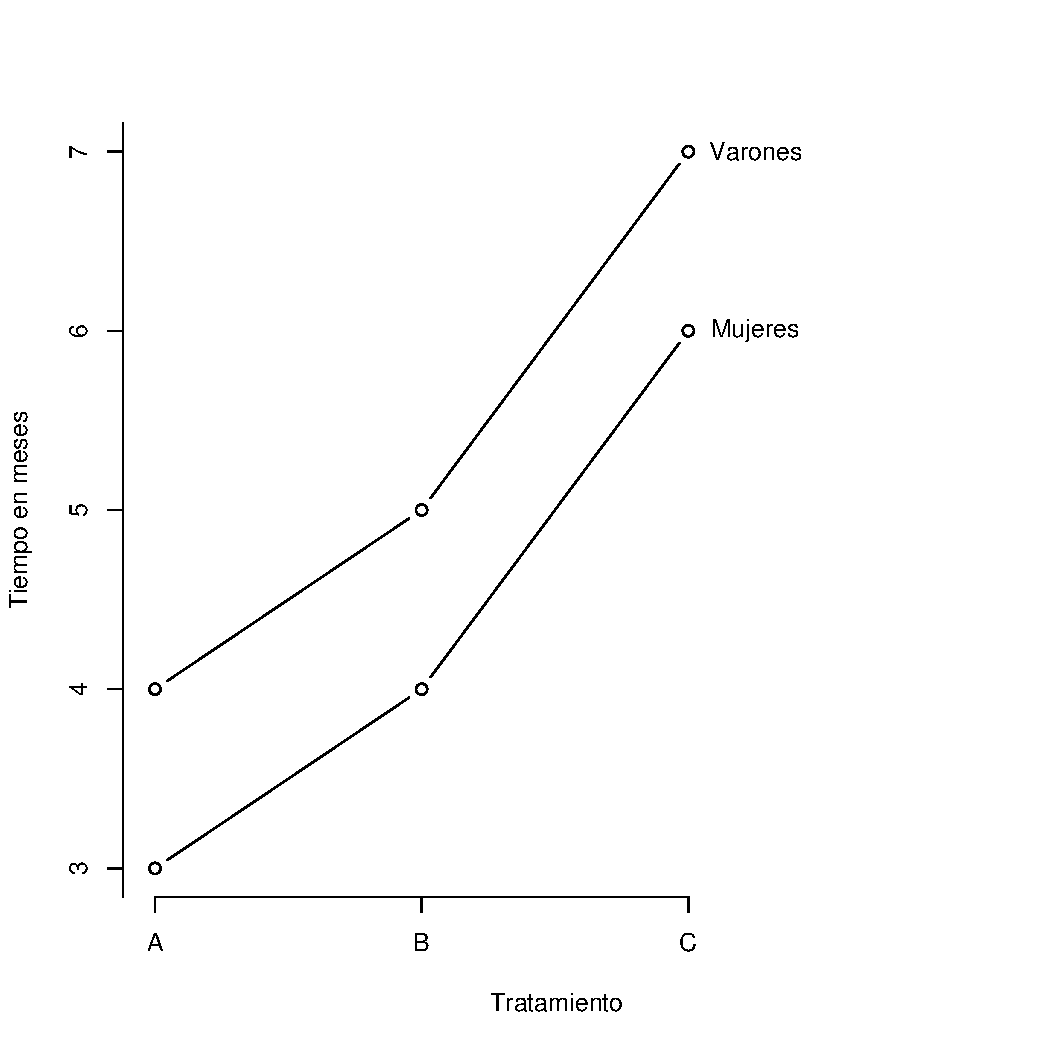
\includegraphics[height=4cm]{NoInteraccio.pdf} 
\end{center}
\item<3-> Diremos que cuando dicho efecto ocurre, no hay interacción entre los bloques y los tratamientos.
\end{itemize}
\end{frame}
%\subsection{Estadísticos muestrales}
\begin{frame}
\frametitle{Estadísticos muestrales}
\begin{itemize}
\item<2-> Se introducen los siguientes estadísticos muestrales:
\begin{itemize}
\item<3-> $T_{i\bullet} = \sum_{j=1}^b X_{ij}$: suma total de las respuestas al $i$-ésimo tratamiento, $i=1,2,\ldots,k$.
\item<4-> $\overline{X}_{i\bullet} =\frac{T_{i\bullet}}{b}$: media muestral del $i$-ésimo tratamiento, $i=1,2,\ldots,k$.
\item<5-> $T_{\bullet j}=\sum_{i=1}^k X_{ij}$: suma total de las respuestas en el $j$-ésimo bloque, $j=1,2,\ldots,b$.
\item<6-> $\overline{X}_{\bullet j} =\frac{T_{\bullet j}}{k}$: media muestral para el $j$-ésimo bloque, $j=1,2,\ldots,b$.
\item<7-> $T_{\bullet\bullet}=\sum_{i=1}^k\sum_{j=1}^b X_{ij}=\sum_{i=1}^k T_{i\bullet}= \sum_{j=1}^b T_{\bullet j}$: suma total de las respuestas.
\item<8-> $\overline{X}_{\bullet\bullet}=\frac{T_{\bullet\bullet}}{k\cdot b}$: media muestral de todas las respuestas.
\item<9-> $\sum_{i=1}^k\sum_{j=1}^b X_{ij}^2$: suma total de cuadrados de cada respuesta.
\end{itemize}
\end{itemize}
\end{frame}

\begin{frame}
\frametitle{Ejemplo}
{Se realiza un experimento para comparar la energía que se requiere para llevar a cabo tres actividades físicas: correr, pasear y montar en bicicleta. La variable de interés es $X$, número de kilocalorías consumidas por kilómetro  recorrido. Se piensa que las diferencias metabólicas entre los individuos pueden afectar al número de kilocalorías requeridas para llevar a cabo una determinada actividad, y se pretende controlar esta variable extraña. Para hacerlo, se seleccionan ocho individuos. Se le pide a cada uno que corra, camine y recorra en bicicleta una distancia medida, y se determina para cada individuo el número de kilocalorías consumidas por kilómetro durante cada actividad. }
\end{frame}

\begin{frame}
\frametitle{Ejemplo}
Las actividades se realizan en orden aleatorio, con tiempo de recuperación entre una y otra. Cada individuo es utilizado como un bloque. Cada actividad se monitoriza exactamente una vez para cada individuo y de este modo se completa el diseño. Cualquier diferencia en el número medio de kilocalorías consumidas se atribuirá a diferencias entre las actividades mismas, puesto que se ha neutralizado el efecto de las diferencias individuales por medio de la construcción de bloques.

La hipótesis nula es:
$$
H_0 : \mu_{1\bullet} = \mu_{2\bullet} = \mu_{3\bullet}, 
$$
donde $\mu_{i\bullet}$, $i=1,2,3$ representa el número medio de kilocalorías consumidas por kilómetro mientras se corre, se pasea o se monta en bicicleta, respectivamente.
\end{frame}
\begin{frame}
\frametitle{Ejemplo}
En la tabla siguiente se muestran los resultados obtenidos por los ocho individuos:
\begin{center}
\begin{tabular}{cccc}
\hline
&\multicolumn{3}{c}{Tratamiento}\\\hline
Bloque&1 (corriendo)&2 (caminando)&3 (pedaleando)\\\hline
1&1.4&1.1&0.7\\
2&1.5&1.2&0.8\\
3&1.8&1.3&0.7\\
4&1.7&1.3&0.8\\
5&1.6&0.7&0.1\\
6&1.5&1.2&0.7\\
7&1.7&1.1&0.4\\
8&2.0&1.3&0.6\\\hline		
\end{tabular}
\end{center}
\end{frame}
\begin{frame}[fragile]
\frametitle{Ejemplo}
\begin{itemize}
\item<2-> Almacenamos los datos en la variable {\tt kilocal} en {\tt R}:

\begin{Schunk}
\begin{Sinput}
> options(width = 50)
> (kilocal <- matrix(c(1.4, 1.1, 0.7, 1.5, 
+     1.2, 0.8, 1.8, 1.3, 0.7, 1.7, 1.3, 
+     0.8, 1.6, 0.7, 0.1, 1.5, 1.2, 0.7, 
+     1.7, 1.1, 0.4, 2, 1.3, 0.6), 8, 3, 
+     byrow = T))
\end{Sinput}
\begin{Soutput}
     [,1] [,2] [,3]
[1,]  1.4  1.1  0.7
[2,]  1.5  1.2  0.8
[3,]  1.8  1.3  0.7
[4,]  1.7  1.3  0.8
[5,]  1.6  0.7  0.1
[6,]  1.5  1.2  0.7
[7,]  1.7  1.1  0.4
[8,]  2.0  1.3  0.6
\end{Soutput}
\end{Schunk}

\end{itemize}
\end{frame}
\begin{frame}[fragile]
\frametitle{Ejemplo}
\begin{itemize}
\item<2-> De cara a trabajar cómodamente vamos a ``apilar'' la variable anterior de la forma siguiente:

{\small 
\begin{Schunk}
\begin{Sinput}
> kilocal2 <- matrix(kilocal, 24, 1)
\end{Sinput}
\end{Schunk}

\begin{verbatim}
     [,1]
 [1,]  1.4
 [2,]  1.5
 [3,]  1.8
 [4,]  1.7
 [5,]  1.6
 [6,]  1.5
 [7,]  1.7
 [8,]  2.0
 [9,]  1.1
[10,]  1.2
[11,]  1.3
[12,]  1.3
[13,]  0.7
[14,]  1.2
...
\end{verbatim}}
\end{itemize}
\end{frame}
\begin{frame}[fragile]
\frametitle{Ejemplo}
\begin{itemize}
\item<2-> Añadimos dos variables más que nos dirán el bloque y el tratamiento al que pertenece cada valor de la variable anterior {\tt kilocal2}:

\begin{Schunk}
\begin{Sinput}
> options(width = 60)
> (bloques <- rep(seq(1:8), 3))
\end{Sinput}
\begin{Soutput}
 [1] 1 2 3 4 5 6 7 8 1 2 3 4 5 6 7 8 1 2 3 4 5 6 7 8
\end{Soutput}
\begin{Sinput}
> (tratam <- c(rep(1, 8), rep(2, 8), rep(3, 8)))
\end{Sinput}
\begin{Soutput}
 [1] 1 1 1 1 1 1 1 1 2 2 2 2 2 2 2 2 3 3 3 3 3 3 3 3
\end{Soutput}
\end{Schunk}

\end{itemize}
\end{frame}
\begin{frame}[fragile]
\frametitle{Ejemplo}
\begin{itemize}
\item<2-> A continuación añadimos como columnas las dos variables anteriores a la variable {\tt kilocal2}:

{\footnotesize
\begin{Schunk}
\begin{Sinput}
> bloques <- as.factor(bloques)
> tratam <- as.factor(tratam)
> kilocal2 <- cbind(kilocal2, tratam, bloques)
\end{Sinput}
\end{Schunk}

\begin{verbatim}
          tratam bloques
 [1,] 1.4      1       1
 [2,] 1.5      1       2
 [3,] 1.8      1       3
 [4,] 1.7      1       4
 [5,] 1.6      1       5
 [6,] 1.5      1       6
 [7,] 1.7      1       7
 [8,] 2.0      1       8
 [9,] 1.1      2       1
[10,] 1.2      2       2
[11,] 1.3      2       3
[12,] 1.3      2       4
[13,] 0.7      2       5
...
\end{verbatim}}
\end{itemize}
\end{frame}
\begin{frame}[fragile]
\frametitle{Ejemplo}
Calculemos los estadísticos para nuestro ejemplo:
{\footnotesize\begin{itemize}
\item<3-> Sumas por bloques:

\begin{Schunk}
\begin{Sinput}
> num_bloques <- 8
> num_tratam <- 3
> sumas_por_bloques <- c()
> for (i in 1:num_bloques) {
+     sumas_por_bloques <- c(sumas_por_bloques, 
+         sum(kilocal2[bloques == i, 1]))
+ }
> sumas_por_bloques
\end{Sinput}
\begin{Soutput}
[1] 3.2 3.5 3.8 3.8 2.4 3.4 3.2 3.9
\end{Soutput}
\end{Schunk}

\item<4-> Sumas por tratamientos:

\begin{Schunk}
\begin{Sinput}
> sumas_por_tratam <- c()
> for (i in 1:num_tratam) {
+     sumas_por_tratam <- c(sumas_por_tratam, sum(kilocal2[tratam == 
+         i, 1]))
+ }
> sumas_por_tratam
\end{Sinput}
\begin{Soutput}
[1] 13.2  9.2  4.8
\end{Soutput}
\end{Schunk}

\end{itemize}}
\end{frame}
\begin{frame}[fragile]
\frametitle{Ejemplo}
\begin{itemize}
\item<2-> Medias por bloques:

{\small
\begin{Schunk}
\begin{Sinput}
> medias_por_bloques <- c()
> for (i in 1:num_bloques) {
+     medias_por_bloques <- c(medias_por_bloques, 
+         mean(kilocal2[bloques == i, 1]))
+ }
> medias_por_bloques
\end{Sinput}
\begin{Soutput}
[1] 1.066667 1.166667 1.266667 1.266667 0.800000 1.133333
[7] 1.066667 1.300000
\end{Soutput}
\end{Schunk}
}

\item<3-> Medias por tratamientos:
{\small
\begin{Schunk}
\begin{Sinput}
> medias_por_tratam <- c()
> for (i in 1:num_tratam) {
+     medias_por_tratam <- c(medias_por_tratam, 
+         mean(kilocal2[tratam == i, 1]))
+ }
> medias_por_tratam
\end{Sinput}
\begin{Soutput}
[1] 1.65 1.15 0.60
\end{Soutput}
\end{Schunk}
}



\end{itemize}
\end{frame}

\begin{frame}[fragile]
\frametitle{Ejemplo}
\begin{itemize}
\item<2-> Suma total:
{
\begin{Schunk}
\begin{Sinput}
> (suma_total <- sum(kilocal2[, 1]))
\end{Sinput}
\begin{Soutput}
[1] 27.2
\end{Soutput}
\end{Schunk}
}

\item<3-> Media total:
{
\begin{Schunk}
\begin{Sinput}
> (media_total <- mean(kilocal2[, 1]))
\end{Sinput}
\begin{Soutput}
[1] 1.133333
\end{Soutput}
\end{Schunk}
}
\end{itemize}
\end{frame}

%\subsection{Suma de cuadrados}
\begin{frame}
\frametitle{Identidad de la suma de cuadrados}
{
\begin{itemize}
\item<2-> Se cumple la igualdad siguiente:
\[
\begin{array}{l}
\sum\limits_{i=1}^k\sum\limits_{j=1}^b (X_{ij}- \overline{X}_{\bullet\bullet})^2 =  \sum\limits_{i=1}^k\sum\limits_{j=1}^b (X_{i\bullet}-\overline{X}_{\bullet\bullet})^2 \\ + \sum\limits_{i=1}^k\sum\limits_{j=1}^b (X_{\bullet j}-\overline{X}_{\bullet\bullet})^2 \\ + \sum\limits_{i=1}^k\sum\limits_{j=1}^b (X_{ij} - X_{i\bullet}- X_{\bullet j}+\overline{X}_{\bullet\bullet})^2,
\end{array}
\]
donde
\end{itemize}}
\end{frame}
\begin{frame}
\frametitle{Identidad de la suma de cuadrados}
{
\begin{itemize}
\item<2-> $SS_{Total} = \sum\limits_{i=1}^k\sum\limits_{j=1}^b (X_{ij}- \overline{X}_{\bullet\bullet})^2$: variabilidad total de los datos.
\item<3-> $SS_{Tr}=\sum\limits_{i=1}^k\sum\limits_{j=1}^b (X_{i\bullet}-\overline{X}_{\bullet\bullet})^2= b \sum\limits_{i=1}^k (X_{i\bullet}-\overline{X}_{\bullet\bullet})^2$: variabilidad de los datos atribuible a la utilización de distintos tratamientos.
\item<4-> $SS_{Bloques}=\sum\limits_{i=1}^k\sum\limits_{j=1}^b (X_{\bullet j}-\overline{X}_{\bullet\bullet})^2=k \sum\limits_{j=1}^b (X_{\bullet j}-\overline{X}_{\bullet\bullet})^2 $: variabilidad de los datos atribuible a la utilización de bloques diferentes.
\item<5-> $SS_E= \sum\limits_{i=1}^k\sum\limits_{j=1}^b (X_{ij} - X_{i\bullet}- X_{\bullet j}+\overline{X}_{\bullet\bullet})^2$: variabilidad de los datos debida a factores aleatorios.
\end{itemize}}
\end{frame}

\begin{frame}[fragile]
\frametitle{Ejemplo}
\begin{itemize}
\item<2-> Calculemos las sumas de cuadrados para nuestro ejemplo:
\begin{itemize}
\item<3-> Variabilidad total:

\begin{Schunk}
\begin{Sinput}
> (SS_total <- sum((kilocal2[, 1] - media_total)^2))
\end{Sinput}
\begin{Soutput}
[1] 5.353333
\end{Soutput}
\end{Schunk}

\item<4-> Variabilidad debida a tratamientos:

\begin{Schunk}
\begin{Sinput}
> (SS_Tr <- num_bloques * sum((medias_por_tratam - 
+     media_total)^2))
\end{Sinput}
\begin{Soutput}
[1] 4.413333
\end{Soutput}
\end{Schunk}

\item<5-> Variabilidad debida a bloques:

\begin{Schunk}
\begin{Sinput}
> (SS_Bl <- num_tratam * sum((medias_por_bloques - 
+     media_total)^2))
\end{Sinput}
\begin{Soutput}
[1] 0.5533333
\end{Soutput}
\end{Schunk}

\end{itemize}
\end{itemize}
\end{frame}
\begin{frame}[fragile]
\frametitle{Ejemplo}
\begin{itemize}
\item<2-> Variabilidad debido al error aleatorio. 
Creamos dos variables auxiliares {\tt aux} y {\tt aux2} para poder realizar la suma usando las medias por tratamientos y por bloques:
{\small

\begin{Schunk}
\begin{Sinput}
> options(width = 60)
> aux <- c()
> for (i in 1:num_tratam) {
+     aux <- c(aux, rep(medias_por_tratam[i], num_bloques))
+ }
> aux
\end{Sinput}
\begin{Soutput}
 [1] 1.65 1.65 1.65 1.65 1.65 1.65 1.65 1.65 1.15 1.15 1.15
[12] 1.15 1.15 1.15 1.15 1.15 0.60 0.60 0.60 0.60 0.60 0.60
[23] 0.60 0.60
\end{Soutput}
\begin{Sinput}
> (aux2 <- rep(medias_por_bloques, num_tratam))
\end{Sinput}
\begin{Soutput}
 [1] 1.066667 1.166667 1.266667 1.266667 0.800000 1.133333
 [7] 1.066667 1.300000 1.066667 1.166667 1.266667 1.266667
[13] 0.800000 1.133333 1.066667 1.300000 1.066667 1.166667
[19] 1.266667 1.266667 0.800000 1.133333 1.066667 1.300000
\end{Soutput}
\end{Schunk}
}
\end{itemize}
\end{frame}
\begin{frame}[fragile]
\frametitle{Ejemplo}
\begin{itemize}
\item<2-> A continuación calculamos la variabilidad del error:

\begin{Schunk}
\begin{Sinput}
> options(width = 50)
> (SS_E <- sum((kilocal2[, 1] - aux - aux2 + 
+     media_total)^2))
\end{Sinput}
\begin{Soutput}
[1] 0.3866667
\end{Soutput}
\end{Schunk}

\item<3-> Podemos comprobar que se verifica:
\[
SS_{Total} = SS_{Tr}+SS_{Bloques}+SS_E.
\]
\end{itemize}
\end{frame}
\subsection{Estadísticos de contraste}
\begin{frame}
\frametitle{Contraste a realizar y estadísticos de contraste}
\begin{itemize}
\item<2-> Para contrastar si existen diferencias entre los tratamientos, tenemos que realizar el contraste siguiente:
\[
\left.
\begin{array}{rl}
H_0 : & \mu_{1\bullet}=\ldots =\mu_{k\bullet}, \\
H_1 : &\exists i,j=1,\ldots ,k\ |\ \mu_{i\bullet}\not = \mu_{j\bullet}.
\end{array}
\right\}
\]
\item<3-> Para realizar el contraste anterior, introducimos los estadísticos siguientes:
\begin{itemize}
\item<4-> Cuadrado medio de los tratamientos: $MS_{Tr}=\frac{SS_{Tr}}{k-1}$.
\item<5-> Cuadrado medio de los bloques: $MS_{Bloques}=\frac{SS_{Bloques}}{b-1}$.
\item<6-> Cuadrado medio del error: $MS_E = \frac{SS_E}{(b-1) (k-1)}$.
\end{itemize}
\end{itemize}
\end{frame}
\begin{frame}
\frametitle{Estadísticos de contraste}
\begin{itemize}
\item<2-> Los valores esperados de los cuadrados medios son:
\[
E(MS_{Tr})=\sigma^2 + \frac{b}{k-1}\sum_{i=1}^k (\mu_{i\bullet}-\mu)^2, \ E(MS_E)=\sigma^2.
\]
\item<3-> Para el contraste anterior, usamos como estadístico de contraste el cociente siguiente:
\[
F=\frac{MS_{Tr}}{MS_E},
\]
que, si $H_0$ es cierta, sigue la distribución $F_{k-1,(k-1) (b-1)}$ (distribución F de Fisher-Snédecor con $k-1$ y $(k-1) (b-1)$ grados de libertad) ya que, en este caso, $\sum_{i=1}^k (\mu_{i\bullet}-\mu)^2 =0$ y tanto $MS_{Tr}$ como $MS_E$ estiman $\sigma^2$. Si $H_0$ no fuese cierta, el valor del estadístico anterior sería mayor que~$1$.
\end{itemize}
\end{frame}

\begin{frame}
\frametitle{Tabla del contraste}
\begin{itemize}
\item<2-> Para realizar el contraste se construye la tabla siguiente donde se ha indicado el método de cálculo para calcular los estadísticos:
{\footnotesize\begin{center}
\begin{tabular}{|@{}l@{}|l@{}|l@{}|l@{}|l|}
\hline
Fuente de&Grados de&Suma de&Cuadrados&Estadístico\\
variación&libertad&cuadrados&medios&\\\hline
Tratam.&$k-1$&$\sum\limits_{i=1}^k \frac{T_{i\bullet}}{b}-\frac{T_{\bullet\bullet}^2}{k\cdot b}$&$\frac{SS_{Tr}}{k-1}$&$\frac{MS_{Tr}}{MS_E}$\\
Bloque&$b-1$&$\sum\limits_{j=1}^b \frac{T_{\bullet j}}{k}-\frac{T_{\bullet\bullet}^2}{k\cdot b}$&$\frac{SS_{Bloques}}{b-1}$&\\
Error&$(k-1)(b-1)$&$SS_{Total}-SS_{Tr}-$&$\frac{SS_E}{(k-1)(b-1)}$&\\
&&$SS_{Bloques}$&&\\\hline
Total&$kb-1$&$\sum\limits_{i=1}^k\sum\limits_{j=1}^b X_{ij}^2-\frac{T_{\bullet\bullet}^2}{k\cdot b}$&&\\\hline
\end{tabular}
\end{center}}
\end{itemize}
\end{frame}
\begin{frame}[fragile]
\frametitle{Ejemplo}
\begin{itemize}
\item<2-> Calculemos la tabla ANOVA para nuestro ejemplo.
\item<3-> En primer lugar, volvemos a calcular las sumas de cuadrados usando las reglas de cálculo vistas anteriormente:
\end{itemize}
\end{frame}

\begin{frame}[fragile]
\frametitle{Ejemplo}
{\footnotesize\begin{itemize}
\item<2-> Sumas de cuadrados por tratamientos:

\begin{Schunk}
\begin{Sinput}
> options(width = 60)
> (SS_Tr <- (1/num_bloques) * sum(sumas_por_tratam^2) - 
+     suma_total^2/(num_bloques * num_tratam))
\end{Sinput}
\begin{Soutput}
[1] 4.413333
\end{Soutput}
\end{Schunk}

\item<3-> Suma de cuadrados por bloques:
\begin{Schunk}
\begin{Sinput}
> options(width = 60)
> (SS_Bl <- (1/num_tratam) * sum(sumas_por_bloques^2) - 
+     suma_total^2/(num_bloques * num_tratam))
\end{Sinput}
\begin{Soutput}
[1] 0.5533333
\end{Soutput}
\end{Schunk}

\item<4-> Suma de cuadrados de error:

\begin{Schunk}
\begin{Sinput}
> options(width = 45)
> (SS_E <- sum(kilocal2[, 1]^2) - suma_total^2/(num_bloques * 
+     num_tratam) - SS_Tr - SS_Bl)
\end{Sinput}
\begin{Soutput}
[1] 0.3866667
\end{Soutput}
\end{Schunk}

\end{itemize}}
\end{frame}
\begin{frame}[fragile]
\frametitle{Ejemplo}
\begin{itemize}
\item<2-> A continuación hacemos la tabla ANOVA:
{\footnotesize\begin{center}
\begin{tabular}{|l@{}|l@{}|l@{}|l@{}|l|}
\hline
Fuente de&Grados de&Suma de&Cuadrados&Estadístico\\
variación&libertad&cuadrados&medios&\\\hline
Tratamiento&$2$&$4.413$&$\frac{4.413}{2}=2.207$&$\frac{2.207}{0.028}=79.897$\\
Bloque&$7$&$0.553$&$\frac{0.553}{7}=0.079$&\\
Error&$14$&$0.387$&$\frac{0.387}{14}=0.028$&\\\hline
Total&$23$&$5.353$&&\\\hline
\end{tabular}
\end{center}}
\item<3-> A un nivel de significación $\alpha =0.05$ buscamos el valor crítico $F_{0.95,2,14}$:

\begin{Schunk}
\begin{Sinput}
> qf(0.95, 2, 14)
\end{Sinput}
\begin{Soutput}
[1] 3.738892
\end{Soutput}
\end{Schunk}

\end{itemize}
\end{frame}
\begin{frame}[fragile]
\frametitle{Ejemplo}
\begin{itemize}
\item<2-> Como el valor del estadístico de contraste, $79.897$, es mayor que el valor crítico, $3.739$, rechazamos la hipótesis nula y concluimos que hay diferencias en la energía media requerida dependiendo de las actividades físicas.
\item<3-> Si hallamos el p-valor del contraste, éste vale:

\begin{Schunk}
\begin{Sinput}
> 1 - pf(79.896, 2, 14)
\end{Sinput}
\begin{Soutput}
[1] 2.201343e-08
\end{Soutput}
\end{Schunk}

valor muy pequeño que nos reafirma en la decisión de rechazar la hipótesis nula.
\end{itemize}
\end{frame}
\begin{frame}[fragile]
\frametitle{Ejemplo}
\begin{itemize}
\item<2-> En {\tt R} se puede realizar el contraste ANOVA directamente:
{\small
\begin{Schunk}
\begin{Sinput}
> options(width = 70)
> summary(aov(kilocal2[, 1] ~ tratam + bloques))
\end{Sinput}
\begin{Soutput}
            Df Sum Sq Mean Sq F value    Pr(>F)    
tratam       2 4.4133 2.20667 79.8966 2.201e-08 ***
bloques      7 0.5533 0.07905  2.8621   0.04462 *  
Residuals   14 0.3867 0.02762                      
---
Signif. codes:  0 ‘***’ 0.001 ‘**’ 0.01 ‘*’ 0.05 ‘.’ 0.1 ‘ ’ 1 
\end{Soutput}
\end{Schunk}
}

\end{itemize}
\end{frame}
\subsection{Construcción de los bloques}
\begin{frame}
\frametitle{Efectividad en la construcción de los bloques}
\begin{itemize}
\item<2-> Nos podemos preguntar si la elección de los bloques ha sido efectiva para nuestro experimento.
\item<3-> Si la respuesta es afirmativa, la variabilidad debida a los bloques, $SS_{Bloques}$, explicaría una parte importante de la suma total de cuadrados. Este hecho, hace que el valor de la variabilidad del error, $SS_E$, disminuya, aumentando el valor del estadístico de contraste $F$ y haciendo más difícil aceptar la hipótesis nula~$H_0$. En este caso, se mejoraría la potencia del contraste.
\item<4-> Para averiguar la efectividad de la construcción de los bloques, se estima lo que se denomina la eficacia relativa ($RE$) del diseño de bloque completo aleatorizado comparada con la del diseño completo aleatorizado visto en secciones anteriores.
\item<5-> La eficacia relativa $RE$ se interpreta com el número de observaciones necesario para que los dos diseños sean equivalentes.
\end{itemize}
\end{frame}
\begin{frame}
\frametitle{Efectividad en la construcción de los bloques}
\begin{itemize}
\item<2-> Por ejemplo, si $RE=3$, significa que el diseño completo aleatorizado requiere tres veces tantas observaciones como el diseño de bloque completo aleatorizado para producir un contraste con las mismas características. En este caso, sería deseable la construcción de bloques. En cambio, si $RE=0.5$, entonces la construcción de bloques no es deseable.
\item<3-> Si $RE=1$, los dos métodos son equivalentes cuando los tamaños muestrales son idénticos.
\item<4-> La manera de estimar $RE$ es la siguiente:
\[
\hat{RE}=c+(1-c)\frac{MS_{bloques}}{MS_E},
\]
donde $c=b(k-1)/(bk-1)$.
\item<5-> Si $\hat{RE}$ nos ha dado un valor mayor que~$1$, significa que la construcción de los bloques ha sido provechosa.
\end{itemize}
\end{frame}
\begin{frame}[fragile]
\frametitle{Ejemplo}
{\small\begin{itemize}
\item<2-> En nuestro caso el valor de $\hat{RE}$ vale:

\begin{Schunk}
\begin{Sinput}
> options(width = 50)
> (valor_c <- num_bloques * (num_tratam - 
+     1)/(num_bloques * num_tratam - 1))
\end{Sinput}
\begin{Soutput}
[1] 0.6956522
\end{Soutput}
\begin{Sinput}
> (MS_Bl <- SS_Bl/(num_bloques - 1))
\end{Sinput}
\begin{Soutput}
[1] 0.07904762
\end{Soutput}
\begin{Sinput}
> (MS_E <- SS_E/((num_bloques - 1) * (num_tratam - 
+     1)))
\end{Sinput}
\begin{Soutput}
[1] 0.02761905
\end{Soutput}
\begin{Sinput}
> (RE <- valor_c + (1 - valor_c) * +MS_Bl/MS_E)
\end{Sinput}
\begin{Soutput}
[1] 1.566717
\end{Soutput}
\end{Schunk}

\item<3-> Al darnos un valor mayor que $1$, concluimos que la construcción de bloques ha sido útil en nuestro caso.
\end{itemize}}
\end{frame}
\subsection{Comparaciones}
\begin{frame}
\frametitle{Comparaciones por parejas y múltiples}
\begin{itemize}
\item<2-> En el caso en que hayamos rechazamos la hipótesis nula, podemos estar interesados en averiguar qué tratamientos son los que difieren.
\item<3-> Al igual que hacíamos en la clasificación de una vía, en este caso también podemos realizar $\binom{k}{2}$ contrastes $t$ de Bonferroni con el nivel de significación~$\alpha$ elegido de tal forma que $\alpha'$, la probabilidad de realizar un contraste incorrecto, se mantenga bajo control.
\item<4-> También podemos realizar un contraste de Duncan de rango múltiple con $SSR_p =r_p \sqrt{\frac{MS_E}{b}}$, donde $p$ es el tamaño del subconjunto de medias muestrales elegido.
\end{itemize}
\end{frame}
\begin{frame}[fragile]
\frametitle{Ejemplo}
\begin{itemize}
\item<2-> Vamos a realizar el contraste de Duncan de rango múltiple para nuestro ejemplo.
\item<3-> Recordemos que las medias por tratamientos eran:
\[
\overline{X}_{1\bullet} =1.65,\ \overline{X}_{2\bullet}=1.15,\ \overline{X}_{3\bullet}=0.60.
\]
\item<4-> A continuación, ordenamos las medias anteriores: $\overline{X}_{3\bullet} < \overline{X}_{2\bullet} < \overline{X}_{1\bullet}$.
\item<5-> Podemos considerar las medias siguientes:
\begin{itemize}
\item<6-> $\overline{X}_{1\bullet} - \overline{X}_{3\bullet}$ ($p=3$).
\item<7-> $\overline{X}_{1\bullet} - \overline{X}_{2\bullet}$ ($p=2$).
\item<8-> $\overline{X}_{2\bullet} - \overline{X}_{3\bullet}$ ($p=2$).
\end{itemize}
\item<9-> La tabla de los valores de $r_p$ y $SSR_p$ para $\alpha =0.05$ es la siguiente (cogemos $14$ como grados de libertad del error):
\begin{center}
\begin{tabular}{|r|r|r|}
\hline
$p$&$2$&$3$\\\hline
$r_p$&3.033&3.178\\\hline
$SSR_p$&0.178&0.187\\\hline
\end{tabular}
\end{center}
\end{itemize}
\end{frame}
\begin{frame}[fragile]
\frametitle{Ejemplo}
\begin{itemize}
\item<2-> Para calcular la tabla anterior, hemos usado el siguiente código~{\tt R}:

\begin{Schunk}
\begin{Sinput}
> rp <- c(3.033, 3.178)
> (SSR_p <- rp * sqrt(MS_E/num_bloques))
\end{Sinput}
\begin{Soutput}
[1] 0.1782099 0.1867296
\end{Soutput}
\end{Schunk}

\item<3-> Veamos en qué tratamientos hay diferencias:
{\small
\begin{center}
\begin{tabular}{|c|c|c|c|c|c|}
\hline
Diferencias&$d$&$p$&$SSR_p$&¿$d>SSR_p$?&Conclusión\\\hline
$\overline{X}_{1\bullet}-\overline{X}_{3\bullet}$&$1.05$&$3$&$0.187$&Sí&$\mu_{1\bullet}\not=\mu_{3\bullet}$\\\hline
$\overline{X}_{1\bullet}-\overline{X}_{2\bullet}$&$0.50$&$2$&$0.178$&Sí&$\mu_{1\bullet}\not=\mu_{2\bullet}$\\\hline
$\overline{X}_{2\bullet}-\overline{X}_{3\bullet}$&$0.55$&$2$&$0.178$&Sí&$\mu_{2\bullet}\not=\mu_{3\bullet}$\\\hline
\end{tabular}
\end{center}
}
\item<4-> Concluimos que las medias de los tres tratamientos son diferentes a un nivel de significación de $0.05$.
\end{itemize}
\end{frame}
\section{Experimentos factoriales}
\begin{frame}
\frametitle{Introducción}
\begin{itemize}
\item<2-> Vamos a generalizar el estudio que hemos realizado hasta ahora en el sentido de que consideraremos que los valores experimentales de los individuos pueden depender de dos o más variables.
\item<3-> Si éste es el caso, el experimento se denomina {\bf experimento factorial.}
\item<4-> En este curso, estudiaremos la clasificación de dos vías, diseño completamente aleatorio con efectos fijos.
\item<5-> Por tanto, en nuestro modelo tendremos dos factores, $A$ y $B$ donde el experimentador ha seleccionado los niveles de cada factor. (efectos fijos)
\end{itemize}
\end{frame}
\begin{frame}
\frametitle{Formato de los datos y notación}
\begin{itemize}
\item<2-> Como hemos comentado anteriormente, consideraremos que el experimento depende de dos factores, $A$ y $B$.
\item<3-> Supondremos que el factor $A$ tiene $a$ niveles y el factor $B$, $b$ niveles. 
\item<4-> El número total de combinaciones de tratamientos o niveles será: $a\cdot b$.
\item<5-> Supondremos que tenemos $n$ observaciones para cada combinación de tratamientos. Por tanto, el número total de observaciones será: $N= n\cdot a\cdot b$.
\item<6-> La variable $X_{ijk}$, $i=1,\ldots,a$, $j=1,\ldots,b$, $k=1,\ldots,n$ es una variables aleatoria que nos da la respuesta de la $k$-ésima unidad experimental al $i$-ésimo nivel del factor~$A$ y del $j$-ésimo nivel del factor~$B$.
\end{itemize}
\end{frame}
\begin{frame}
\frametitle{Formato de los datos y notación}
{Todo queda reflejado en la tabla siguiente:} 
{\small\begin{center}
\begin{tabular}{ccccc}
\hline
&\multicolumn{4}{c}{Nivel del factor $A$}\\\hline
Factor $B$&$1$&$2$&$\cdots$&$a$\\\hline
$1$&$X_{111}$&$X_{211}$&$\cdots$&$X_{a11}$\\
&$X_{112}$&$X_{212}$&$\cdots$&$X_{a12}$\\
&$\cdots$&$\cdots$&$\cdots$&$\cdots$\\
&$X_{11n}$&$X_{21n}$&$\cdots$&$X_{a1n}$\\\hline
$2$&$X_{121}$&$X_{221}$&$\cdots$&$X_{a21}$\\
&$X_{122}$&$X_{222}$&$\cdots$&$X_{a22}$\\
&$\cdots$&$\cdots$&$\cdots$&$\cdots$\\
&$X_{12n}$&$X_{22n}$&$\cdots$&$X_{a2n}$\\\hline
$\vdots$&$\vdots$&$\vdots$&$\vdots$&$\vdots$\\\hline
$b$&$X_{1b1}$&$X_{2b1}$&$\cdots$&$X_{ab1}$\\
&$X_{1b2}$&$X_{2b2}$&$\cdots$&$X_{ab2}$\\
&$\cdots$&$\cdots$&$\cdots$&$\cdots$\\
&$X_{1bn}$&$X_{2bn}$&$\cdots$&$X_{abn}$\\\hline
\end{tabular}
\end{center}}
\end{frame}
\subsection{Modelo}
\begin{frame}
\frametitle{Modelo}
{\small
\begin{itemize}
\item<2-> El modelo es el siguiente:
\[
\begin{array}{l}
X_{ijk} = \mu + \alpha_i + \beta_j + (\alpha\beta)_{ij}+E_{ijk},\\
i=1,\ldots,a,\ j=1,\ldots,b,\ k=1,\ldots,n,
\end{array}\]
\item<3-> donde
\begin{itemize}
\item<4-> $\mu$: efecto medio global,
\item<5-> $\mu_{i\bullet\bullet}$: media para el $i$-ésimo nivel del factor~$A$.
\item<6-> $\mu_{\bullet j\bullet}$: media para el $j$-ésimo nivel del factor~$B$.
\item<7-> $\mu_{ij\bullet}$: media para la $i-j$-ésima combinación de tratamientos.
\item<8-> $\alpha_i =\mu_{i\bullet\bullet}-\mu$: efecto debido al hecho de que la unidad experimental está en el $i$-ésimo nivel del factor~$A$.
\item<9-> $\beta_j =\mu_{\bullet j\bullet}-\mu$: efecto debido al hecho de que la unidad experimental está en el $j$-ésimo nivel del factor~$B$.
\item<10-> $(\alpha\beta)_{ij}=\mu_{ij\bullet}-\mu_{i\bullet\bullet}-\mu_{\bullet j\bullet}+\mu$: efecto de interacción entre el $i$-ésimo nivel del factor~$A$ y el $j$-ésimo nivel del factor~$B$.
\item<11-> $E_{ijk}=X_{ijk}-\mu_{ij\bullet}$: error residual o aleatorio.
\end{itemize}
\end{itemize}}
\end{frame}
\begin{frame}
\frametitle{Supuestos del modelo}
\begin{itemize}
\item<2-> Nuestro modelo tiene las suposiciones siguientes:
\begin{itemize}
\item<3-> Las observaciones para cada combinación de tratamientos constituyen muestras aleatorias independientes, cada una de tamaño~$n$, de $a\cdot b$ poblaciones con media $\mu_{ij\bullet}$.
\item<4-> Cada una de las $a\cdot b$ poblaciones es normal.
\item<5-> Cada una de las $a\cdot b$ poblaciones tiene la misma varianza, $\sigma^2$.
\end{itemize}
\end{itemize}
\end{frame}
%\subsection{Estadísticos muestrales}
\begin{frame}
\frametitle{Estadísticos muestrales}
Se introducen los siguientes estadísticos muestrales:
{
\begin{itemize}
\item<2-> $T_{ij\bullet}=\sum\limits_{k=1}^n$: suma total de las respuestas al $i$-ésimo nivel del factor~$A$ y al $j$-ésimo nivel del factor~$B$.
\item<3-> $\overline{X}_{ij\bullet}=\frac{T_{ij\bullet}}{n}$: media muestral para la $i-j$-ésima combinación de tratamientos.
\item<4-> $T_{i\bullet\bullet}=\sum\limits_{j=1}^b T_{ij\bullet}$: suma total de las respuestas al $i$-ésimo nivel del factor~$A$.
\item<5-> $\overline{X}_{i\bullet\bullet}=\frac{T_{i\bullet\bullet}}{bn}$: media muestral para el $i$-ésimo nivel del factor~$A$.
\end{itemize}}
\end{frame}
\begin{frame}
\frametitle{Estadísticos muestrales}
\begin{itemize}
\item<2-> $T_{\bullet j\bullet}=\sum\limits_{i=1}^a T_{ij\bullet}$: suma total de las respuestas al $j$-ésimo nivel del factor~$B$.
\item<3-> $\overline{X}_{\bullet j\bullet}=\frac{T_{\bullet j\bullet}}{an}$: media muestral para el $j$-ésimo nivel del factor~$B$.
\item<4-> $T_{\bullet\bullet\bullet}=\sum\limits_{i=1}^{a} T_{i\bullet\bullet}=\sum\limits_{j=1}^b T_{\bullet j\bullet} =\sum\limits_{i=1}^a\sum\limits_{j=1}^b T_{ij\bullet}$: suma total de las respuestas.
\item<5-> $\overline{X}_{\bullet\bullet\bullet}=\frac{T_{\bullet\bullet\bullet}}{a b n}$: media muestral para todas las respuestas.
\end{itemize}
\end{frame}
\begin{frame}
\frametitle{Ejemplo}
\begin{block}{Estudio del efecto de la luz y la temperatura sobre el crecimiento del ovario del pez {\it Mirogrex terrae-sanctae}}
El {\it Mirogrex terrae-sanctae} es un pez comercializado semejante a la sardina que se encontró en el Mar de Galilea. Se realizó un estudio para determinar el efecto de la luz y la temperatura sobre el índice gonadosomático (GSI), que es una medida de crecimiento del ovario. Se utilizaron dos fotoperíodos: catorce horas de luz, diez horas de oscuridad y nueve horas de luz, quince horas de oscuridad; y dos niveles de temperatura, 16 y 27 ${}^\circ$C. De este modo, el experimentador puede simular situaciones de verano e invierno en la región. Se trata de un experimento factorial con dos factores, luz y temperatura, que son investigados cada uno a dos niveles.
\end{block}
\end{frame}
\begin{frame}
\frametitle{Ejemplo}
\begin{block}{Datos obtenidos}
El experimento se realizó sobre $20$ hembras en junio. Se dividieron aleatoriamente las $20$ hembras en $4$ subgrupos de tamaño~$5$ cada uno. Después de tres meses se determinó el $GSI$ para cada pez. Los resultados se muestran en la tabla siguiente:
{\footnotesize
\begin{center}
\begin{tabular}{ccc}
\hline
&\multicolumn{2}{c}{Factor $A$ (fotoperíodo)}\\\hline
Factor $B$&$9$ horas&$14$ horas\\
(temperatura)&&\\\hline
$27^\circ$C&$0.90$&$0.83$\\
&$1.06$&$0.67$\\
&$0.98$&$0.57$\\
&$1.29$&$0.47$\\
&$1.12$&$0.66$\\\hline
$16^\circ$C&$1.30$&$1.01$\\
&$2.88$&$1.52$\\
&$2.42$&$1.02$\\
&$2.66$&$1.32$\\
&$2.94$&$1.63$\\\hline
\end{tabular}
\end{center}}
\end{block}
\end{frame}
\begin{frame}
\frametitle{Ejemplo. Introducción de los datos en {\tt R}}
\begin{itemize}
\item<2-> En primer lugar, introducimos tres variables:
\begin{enumerate}
\item<3-> {\tt peces} donde introduciremos los valores de la variable $GSI$ de cada pez,
\item<4-> {\tt periodo} donde introduciremos el valor del nivel para el factor $A$ (fotoperíodo) y
\item<5-> {\tt temperatura} donde introduciremos el valor del nivel para el factor $B$ (temperatura).
\end{enumerate}
\end{itemize}
\end{frame}
\begin{frame}[fragile]
\frametitle{Ejemplo. Introducción de los datos en {\tt R}}

{\small
\begin{Schunk}
\begin{Sinput}
> (peces <- c(0.9, 0.83, 1.06, 0.67, 0.98, 0.57, 1.29, 
+     0.47, 1.12, 0.66, 1.3, 1.01, 2.88, 1.52, 2.42, 
+     1.02, 2.66, 1.32, 2.94, 1.63))
\end{Sinput}
\begin{Soutput}
 [1] 0.90 0.83 1.06 0.67 0.98 0.57 1.29 0.47 1.12 0.66 1.30 1.01
[13] 2.88 1.52 2.42 1.02 2.66 1.32 2.94 1.63
\end{Soutput}
\begin{Sinput}
> (periodo <- factor(rep(c(9, 14), 10)))
\end{Sinput}
\begin{Soutput}
 [1] 9  14 9  14 9  14 9  14 9  14 9  14 9  14 9  14 9  14 9  14
Levels: 9 14
\end{Soutput}
\begin{Sinput}
> (temperatura <- factor(c(rep(27, 10), rep(16, 10))))
\end{Sinput}
\begin{Soutput}
 [1] 27 27 27 27 27 27 27 27 27 27 16 16 16 16 16 16 16 16 16 16
Levels: 16 27
\end{Soutput}
\end{Schunk}
}

\end{frame}
\begin{frame}[fragile]
\frametitle{Ejemplo. Introducción de los datos en {\tt R}}
{\small 
A continuación, juntamos las tres variables anteriores en un sólo {\tt data frame} llamado {\tt peces2}:
{\footnotesize
\begin{Schunk}
\begin{Sinput}
> peces2 <- data.frame(peces, periodo, temperatura)
\end{Sinput}
\end{Schunk}

\begin{verbatim}
   peces periodo temperatura
1   0.90       9          27
2   0.83      14          27
3   1.06       9          27
4   0.67      14          27
5   0.98       9          27
6   0.57      14          27
7   1.29       9          27
8   0.47      14          27
9   1.12       9          27
10  0.66      14          27
11  1.30       9          16
12  1.01      14          16
13  2.88       9          16
14  1.52      14          16
15  2.42       9          16
16  1.02      14          16
...
\end{verbatim}}}
\end{frame}
\begin{frame}[fragile]
\frametitle{Ejemplo. Cálculo de los estadísticos muestrales}
{\begin{itemize}
\item<2-> Suma total de las respuestas al nivel $i$-ésimo para el factor $A$ y al nivel $j$-ésimo para el factor~$B$ ($T_{ij\bullet}$):
\begin{Schunk}
\begin{Sinput}
> sumas_A_B <- c()
> for (i in 1:2) {
+     aux <- c()
+     for (j in 1:2) {
+         aux <- c(aux, sum(peces2[periodo == 
+             unique(periodo)[i] & temperatura == 
+             unique(temperatura)[j], 1]))
+     }
+     sumas_A_B <- cbind(sumas_A_B, aux)
+ }
> sumas_A_B
\end{Sinput}
\begin{Soutput}
       aux aux
[1,]  5.35 3.2
[2,] 12.20 6.5
\end{Soutput}
\end{Schunk}

\end{itemize}}
\end{frame}

\begin{frame}[fragile]
\frametitle{Ejemplo. Cálculo de los estadísticos muestrales}
{\begin{itemize}
\item<2-> Media muestral para la $i-j$-ésima combinación de tratamientos ($\overline{X}_{ij\bullet}$):
\begin{Schunk}
\begin{Sinput}
> (medias_A_B <- sumas_A_B/5)
\end{Sinput}
\begin{Soutput}
      aux  aux
[1,] 1.07 0.64
[2,] 2.44 1.30
\end{Soutput}
\end{Schunk}
\end{itemize}}
\end{frame}

\begin{frame}[fragile]
\frametitle{Ejemplo. Cálculo de los estadísticos muestrales}
{\small
\begin{itemize}
\item<2-> Suma total de las respuestas al $i$-ésimo nivel del factor~$A$ ($T_{i\bullet\bullet}$):
\begin{Schunk}
\begin{Sinput}
> sumas_A <- c()
> for (i in 1:2) {
+     sumas_A <- c(sumas_A, sum(peces2[periodo == 
+         unique(periodo)[i], 1]))
+ }
> sumas_A
\end{Sinput}
\begin{Soutput}
[1] 17.55  9.70
\end{Soutput}
\end{Schunk}
\item<3-> Media muestral para el $i$-ésimo nivel del factor~$A$ ($\overline{X}_{i\bullet\bullet}$):
\begin{Schunk}
\begin{Sinput}
> (medias_A <- sumas_A/(5 * 2))
\end{Sinput}
\begin{Soutput}
[1] 1.755 0.970
\end{Soutput}
\end{Schunk}
\end{itemize}}
\end{frame}
\begin{frame}[fragile]
\frametitle{Ejemplo. Cálculo de los estadísticos muestrales}
{\small 
\begin{itemize}
\item<2-> Suma total de las respuestas al $j$-ésimo nivel del factor~$B$ ($T_{\bullet j\bullet}$):
\begin{Schunk}
\begin{Sinput}
> sumas_B <- c()
> for (j in 1:2) {
+     sumas_B <- c(sumas_B, sum(peces2[temperatura == 
+         unique(temperatura)[j], 1]))
+ }
> sumas_B
\end{Sinput}
\begin{Soutput}
[1]  8.55 18.70
\end{Soutput}
\end{Schunk}
\item<3-> Media muestral para el $j$-ésimo nivel del factor~$B$ ($\overline{X}_{\bullet j\bullet}$):
\begin{Schunk}
\begin{Sinput}
> (medias_B <- sumas_B/(5 * 2))
\end{Sinput}
\begin{Soutput}
[1] 0.855 1.870
\end{Soutput}
\end{Schunk}
\end{itemize}}
\end{frame}
\begin{frame}[fragile]
\frametitle{Ejemplo. Cálculo de los estadísticos muestrales}
\begin{itemize}
\item<2-> Suma total de las respuestas ($T_{\bullet\bullet\bullet}$):
\begin{Schunk}
\begin{Sinput}
> (suma_total <- sum(peces2[, 1]))
\end{Sinput}
\begin{Soutput}
[1] 27.25
\end{Soutput}
\end{Schunk}
\item<3-> Media total de las respuestas ($\overline{X}_{\bullet\bullet\bullet}$):
\begin{Schunk}
\begin{Sinput}
> (media_total <- suma_total/(5 * 2 * 2))
\end{Sinput}
\begin{Soutput}
[1] 1.3625
\end{Soutput}
\end{Schunk}
\end{itemize}
\end{frame}



\begin{frame}
\frametitle{Identidad de la suma de cuadrados}
Definimos las sumas de cuadrados siguientes:
\begin{itemize}
\item<2-> Variabilidad total: $SS_{Total} = \sum\limits_{i=1}^a\sum\limits_{j=1}^b\sum\limits_{k=1}^n (X_{ijk}-\overline{X}_{\bullet\bullet\bullet})^2$.
\item<3-> Variabilidad debida a la utilización de diferentes niveles del factor~$A$: $SS_A =b n\sum\limits_{i=1}^a (\overline{X}_{i\bullet\bullet}-\overline{X}_{\bullet\bullet\bullet})^2$.
\item<4-> Variabilidad debida a la utilización de diferentes niveles del factor~$B$: $SS_B =a n\sum\limits_{j=1}^b (\overline{X}_{\bullet j\bullet}-\overline{X}_{\bullet\bullet\bullet})^2$.
\item<5-> Variabilidad debida a la interacción entre niveles de los factores~$A$ y $B$: $SS_{AB}=n \sum\limits_{i=1}^a\sum\limits_{j=1}^b  (X_{ij\bullet}-\overline{X}_{i\bullet\bullet}-\overline{X}_{\bullet j\bullet}+\overline{X}_{\bullet\bullet\bullet})^2$.
\item<6-> Variabilidad debida al error aleatorio: $SS_E = \sum\limits_{i=1}^a\sum\limits_{j=1}^b\sum\limits_{k=1}^n (X_{ijk}-\overline{X}_{ij\bullet})^2$.
\end{itemize}
\end{frame}
\begin{frame}[fragile]
\frametitle{Cáculo de las sumas de cuadrados para el ejemplo}
{\small\begin{itemize}
\item<2-> Variabilidad total, $SS_{Total}$:
\begin{Schunk}
\begin{Sinput}
> (SS_total <- sum((peces2[, 1] - media_total)^2))
\end{Sinput}
\begin{Soutput}
[1] 11.13377
\end{Soutput}
\end{Schunk}
\item<3-> Variabilidad debida al factor~$A$, $SS_A$:
\begin{Schunk}
\begin{Sinput}
> (SS_A <- 2 * 5 * sum((medias_A - media_total)^2))
\end{Sinput}
\begin{Soutput}
[1] 3.081125
\end{Soutput}
\end{Schunk}
\item<4-> Variabilidad debida al factor~$B$, $SS_B$:
\begin{Schunk}
\begin{Sinput}
> (SS_B <- 2 * 5 * sum((medias_B - media_total)^2))
\end{Sinput}
\begin{Soutput}
[1] 5.151125
\end{Soutput}
\end{Schunk}
\end{itemize}}
\end{frame}
\begin{frame}[fragile]
\frametitle{Cáculo de las sumas de cuadrados para el ejemplo}
{\begin{itemize}
\item<2-> Variabilidad debida a la interacción entre $A$ y $B$, $SS_{AB}$:
\begin{Schunk}
\begin{Sinput}
> SS_AB <- 0
> for (i in 1:2) {
+     for (j in 1:2) {
+         SS_AB <- SS_AB + (medias_A_B[j, 
+             i] - medias_A[i] - medias_B[j] + 
+             media_total)^2
+     }
+ }
> (SS_AB <- 5 * SS_AB)
\end{Sinput}
\begin{Soutput}
     aux 
0.630125 
\end{Soutput}
\end{Schunk}
\end{itemize}}
\end{frame}
\begin{frame}[fragile]
\frametitle{Cáculo de las sumas de cuadrados para el ejemplo}
\begin{itemize}
\item<2-> Variabilidad debida al error aleatorio, $SS_E$:
\begin{Schunk}
\begin{Sinput}
> SS_E <- 0
> for (i in 1:2) {
+     for (j in 1:2) {
+         SS_E <- SS_E + sum((peces2[periodo == 
+             unique(periodo)[i] & temperatura == 
+             unique(temperatura)[j], 1] - 
+             medias_A_B[j, i])^2)
+     }
+ }
> SS_E
\end{Sinput}
\begin{Soutput}
[1] 2.2714
\end{Soutput}
\end{Schunk}
\item<3-> Podemos comprobar que se verifica:
\[
SS_{Total} =SS_A + SS_B + SS_{AB} + SS_E.
\]
\end{itemize}
\end{frame}
\begin{frame}
\frametitle{Cálculo de las sumas de cuadrados}
De cara a simplificar los cálculos, se usan las fórmulas siguientes para calcular las sumas de cuadrados:
\begin{itemize}
\item<2-> $SS_A = \frac{1}{bn}\sum\limits_{i=1}^a T_{i\bullet\bullet}^2-\frac{T_{\bullet\bullet\bullet}^2}{abn}$.
\item<3-> $SS_B =\frac{1}{an}\sum\limits_{j=1}^b T_{\bullet j\bullet}^2-\frac{T_{\bullet\bullet\bullet}^2}{abn}$.
\item<4-> $SS_{Total} = \sum\limits_{i=1}^a\sum\limits_{j=1}^b\sum\limits_{k=1}^n X_{ijk}^2 -\frac{T_{\bullet\bullet\bullet}^2}{abn}$.
\item<5-> $SS_{AB} = SS_{Tr} -SS_A-SS_B$,  donde $SS_{Tr}=\frac{1}{n}\sum\limits_{i=1}^a\sum\limits_{j=1}^b T_{ij\bullet}^2 -
\frac{T_{\bullet\bullet\bullet}^2}{abn}$.
\item<6-> $SS_E = SS_{Total}-SS_{Tr}$.
\end{itemize}
\end{frame}
\begin{frame}[fragile]
\frametitle{Ejemplo}
Vamos a usar las fórmulas anteriores para recalcular las sumas de cuadrados:
\begin{itemize}
\item<2-> $SS_A$:
\begin{Schunk}
\begin{Sinput}
> (SS_A <- (1/(2 * 5)) * sum(sumas_A^2) - 
+     (1/(2 * 2 * 5)) * suma_total^2)
\end{Sinput}
\begin{Soutput}
[1] 3.081125
\end{Soutput}
\end{Schunk}
\item<3-> $SS_B$:
\begin{Schunk}
\begin{Sinput}
> (SS_B <- (1/(2 * 5)) * sum(sumas_B^2) - 
+     (1/(2 * 2 * 5)) * suma_total^2)
\end{Sinput}
\begin{Soutput}
[1] 5.151125
\end{Soutput}
\end{Schunk}
\item<4-> $SS_{Total}$:
\begin{Schunk}
\begin{Sinput}
> (SS_total <- sum(peces2[, 1]^2) - (1/(2 * 
+     2 * 5)) * suma_total^2)
\end{Sinput}
\begin{Soutput}
[1] 11.13377
\end{Soutput}
\end{Schunk}
\end{itemize}
\end{frame}
\begin{frame}[fragile]
\frametitle{Ejemplo}
\begin{itemize}
\item<2-> $SS_{AB}$:
\begin{Schunk}
\begin{Sinput}
> (SS_Tr <- (1/5) * sum(sumas_A_B^2) - (1/(2 * 
+     2 * 5)) * suma_total^2)
\end{Sinput}
\begin{Soutput}
[1] 8.862375
\end{Soutput}
\begin{Sinput}
> (SS_AB <- SS_Tr - SS_A - SS_B)
\end{Sinput}
\begin{Soutput}
[1] 0.630125
\end{Soutput}
\end{Schunk}
\item<3-> $SS_E$:
\begin{Schunk}
\begin{Sinput}
> (SS_E <- SS_total - SS_Tr)
\end{Sinput}
\begin{Soutput}
[1] 2.2714
\end{Soutput}
\end{Schunk}
\end{itemize}
\end{frame}
\subsection{Contrastes a realizar}
\begin{frame}
\frametitle{Contrastes a realizar}
\begin{itemize}
\item<2-> Cuando realizamos un experimento factorial de dos vías, hemos de tener en cuenta los contrastes siguientes:
\begin{enumerate}
\item<3-> Contraste de no interacción. Contrastamos que no hay interacción entre los factores~$A$ y $B$:
\[
\left.
\begin{array}{rl}
H_0 : & (\alpha\beta)_{ij} =0,  \\
H_1 : & \exists i,j\ |\ (\alpha\beta)_{ij}\not = 0.
\end{array}
\right\}
\]
\item<4-> Contraste de que no hay diferencias entre los niveles del factor~$A$:
\[
\left.
\begin{array}{rl}
H_0 : &\mu_{1\bullet\bullet}=\mu_{2\bullet\bullet}=\cdots =\mu_{a\bullet\bullet},  \\
H_1 : & \exists i,i'\ |\ \mu_{i\bullet\bullet}\not = \mu_{i'\bullet\bullet}.
\end{array}
\right\}
\]
\item<5-> Contraste de que no hay diferencias entre los niveles del factor~$B$:
\[
\left.
\begin{array}{rl}
H_0 : &\mu_{\bullet 1\bullet}=\mu_{\bullet 2\bullet}=\cdots =\mu_{ \bullet b\bullet},  \\
H_1 : & \exists j,j'\ |\ \mu_{\bullet j\bullet}\not = \mu_{\bullet j'\bullet}.
\end{array}
\right\}
\]
\end{enumerate}
\end{itemize}
\end{frame}
\begin{frame}
\frametitle{Estadísticos de contraste}
Los estadísticos de contraste que vamos a usar en los contrastes anteriores son los siguientes:
\begin{itemize}
\item<2-> Contraste de no interacción. 
\[
F = \frac{MS_{AB}}{MS_E},
\]
donde $MS_{AB}=\frac{SS_{AB}}{(a-1)(b-1)}$, $MS_E=\frac{SS_E}{ab (n-1)}$ y la distribución del estadístico~$F$, si la hipótesis nula es cierta, es la
distribución $F$ de Fisher-Snédecor con $(a-1)(b-1)$ y $ab(n-1)$ grados de libertad ($F_{(a-1)(b-1),ab(n-1)}$).
\end{itemize}
\end{frame}
\begin{frame}
\frametitle{Estadísticos de contraste}
\begin{itemize}
\item<2-> Contraste de que no hay diferencias entre los niveles del factor~$A$:
\[
F=\frac{MS_A}{MS_E},
\]
donde $MS_A =\frac{SS_A}{a-1}$ y el estadístico $F$, si $H_0$ es cierta, sigue la distribución~$F$ de Fisher-Snédecor con $a-1$ y $ab(n-1)$ grados de libertad ($F_{a-1,ab(n-1)}$).
\item<3-> Contraste de que no hay diferencias entre los niveles del factor~$B$:
\[
F=\frac{MS_B}{MS_E},
\]
donde $MS_B =\frac{SS_B}{b-1}$ y el estadístico $F$, si $H_0$ es cierta, sigue la distribución~$F$ de Fisher-Snédecor con $b-1$ y $ab(n-1)$ grados de libertad ($F_{b-1,ab(n-1)}$).
\end{itemize}
\end{frame}
\begin{frame}
\frametitle{Tabla ANOVA}
Los tres contrastes anteriores se resumen en la siguiente tabla:
{\footnotesize
\begin{center}
\begin{tabular}{|@{}l@{}|@{}l@{}|@{}l@{}|@{}l@{}|@{}l@{}|}
\hline
Variación&Grados de&Suma de&Cuadrados&Estadísticos~$F$\\
&libertad&cuadrados&medios&\\\hline
Tratam.&$ab-1$&$SS_{Tr}$&${SS_{Tr}}/{(ab-1)}$&${MS_{Tr}}/{MS_E}$\\
$A$&$a-1$&$SS_A$&${SS_A}/{(a-1)}$&${MS_{A}}/{MS_E}$\\
$B$&$b-1$&$SS_B$&${SS_B}/{(b-1)}$&${MS_{B}}/{MS_E}$\\
$AB$&$(a-1)(b-1)$&$SS_{AB}$&${SS_{AB}}/{((a-1)(b-1))}$&${MS_{AB}}/{MS_E}$\\
Error&$ab(n-1)$&$SS_E$&${SS_E}/{(ab(n-1))}$&\\\hline
Total&$abn-1$&$SS_{Total}$&&\\\hline
\end{tabular}
\end{center}
}
\end{frame}
\begin{frame}
\frametitle{Tabla ANOVA para el ejemplo}
{\footnotesize
\begin{center}
\begin{tabular}{|l|r|l|l|l|}
\hline
Variación&Grados de&Suma de&Cuadrados&Estadísticos~$F$\\
&libertad&cuadrados&medios&\\\hline
Tratam.&$3$&$8.862$&$2.954$&$20.809$\\
$A$&$1$&$3.081$&$3.081$&$21.704$\\
$B$&$1$&$5.151$&$5.151$&$36.285$\\
$AB$&$1$&$0.630$&$0.630$&$4.439$\\
Error&$16$&$2.271$&$0.142$&\\\hline
Total&$19$&$11.134$&&\\\hline
\end{tabular}
\end{center}
}
\end{frame}
\begin{frame}[fragile]
\frametitle{$p$ valores para los contrastes del ejemplo}
Los p-valores para los tres contrastes valen en nuestro ejemplo:
{\footnotesize
\begin{itemize}
\item<2-> Contraste de no interacción entre los factores $A$ y $B$: $p=p(F_{1,16} > 4.439)\approx 0.051$. Es un $p$-valor pequeño. Por tanto, rechazaríamos la hipótesis nula y concluiríamos que sí hay interacción entre el fotoperíodo y la temperatura.
\begin{Schunk}
\begin{Sinput}
> 1 - pf(4.439, 1, 16)
\end{Sinput}
\begin{Soutput}
[1] 0.05126085
\end{Soutput}
\end{Schunk}
\item<3-> Contraste de que no hay diferencias entre los niveles del factor~$A$ (fotoperíodo): $p=p(F_{1,16}>21.704)\approx 0.00026$. Es un valor muy
pequeño; por tanto, rechazamos $H_0$ y concluimos que hay diferencias entre los niveles del fotoperíodo.
\begin{Schunk}
\begin{Sinput}
> 1 - pf(21.704, 1, 16)
\end{Sinput}
\begin{Soutput}
[1] 0.0002621106
\end{Soutput}
\end{Schunk}
\item<4-> Contraste de que no hay diferencias entre los niveles del factor~$B$ (temperatura): $p=p(F_{1,16}>36.285)\approx 0.000018$. Es un valor muy
pequeño; por tanto, rechazamos $H_0$ y concluimos que hay diferencias entre los niveles de la temperatura.
\begin{Schunk}
\begin{Sinput}
> 1 - pf(36.285, 1, 16)
\end{Sinput}
\begin{Soutput}
[1] 1.771135e-05
\end{Soutput}
\end{Schunk}
\end{itemize}}
\end{frame}
\begin{frame}[fragile]
\frametitle{Resultado directo del ejemplo con {\tt R}}
Con {\tt R} podemos obtener la tabla ANOVA anterior directamente:
{\footnotesize
\begin{Schunk}
\begin{Sinput}
> summary(aov(peces2[, 1] ~ periodo * temperatura))
\end{Sinput}
\begin{Soutput}
                    Df Sum Sq Mean Sq F value
periodo              1 3.0811  3.0811 21.7038
temperatura          1 5.1511  5.1511 36.2851
periodo:temperatura  1 0.6301  0.6301  4.4387
Residuals           16 2.2714  0.1420        
                       Pr(>F)    
periodo             0.0002621 ***
temperatura         1.771e-05 ***
periodo:temperatura 0.0512685 .  
Residuals                        
---
Signif. codes:  0 ‘***’ 0.001 ‘**’ 0.01 ‘*’ 0.05 ‘.’ 0.1 ‘ ’ 1 
\end{Soutput}
\end{Schunk}
}
\end{frame}
\subsection{Comparaciones}
\begin{frame}
\frametitle{Comparaciones usando el contraste de Duncan}
\begin{itemize}
\item<2-> En el caso en que hayamos rechazado una (o las dos hipótesis nulas) respecto a las diferencias entre los niveles de los factores~$A$ o $B$,
hemos de ver en qué niveles hay diferencias.
\item<3-> Para hacerlo, podemos usar el contraste de Duncan comentado en secciones anteriores.
\item<4-> En el caso de ver entre qué niveles del factor $A$ hay diferencias, hay que usar el siguiente contraste de Duncan:
\[
SSR_p = r_p \sqrt{\frac{MS_E}{bn}}.
\]
\item<5-> En el caso de ver entre qué niveles del factor $B$ hay diferencias, hay que usar el siguiente contraste de Duncan:
\[
SSR_p = r_p \sqrt{\frac{MS_E}{an}}.
\]
\end{itemize}
\end{frame}
